\chapter{Data Sample and Event Selection}
\label{sec:bsdatasampleAndSelection}
The data sample used for this analysis corresponds to 19.7$\pm0.5~\fbinv$ of integrated 
luminosity collected in 2012 at $\sqrt{s} = 8~\TeV$.  See Table \ref{table:datasets} for a summary of the datasets used in the analysis.

\section{Signal Samples}
\label{sec:bssignal}


The $\bs$ generation is performed using two different coupling hypotheses. 
\begin{itemize}
\item {\bf $\bs_{R}$} - The purely right-handed $\bs$ where $\kappa_{L}^{b}=g_{L}=0$ , $\kappa_{R}^{b}=g_{R}=1$ 
\item {\bf $\bs_{L}$} - The purely left-handed $\bs$ where $\kappa_{L}^{b}=g_{L}=1$ , $\kappa_{R}^{b}=g_{R}=0$ 
\end{itemize}

The right- and left-handed $\bs$ samples used in this analysis are given in table
\ref{table:bssignalsetsright} and \ref{table:bssignalsetsleft} respectively. The vectorlike $\bs_{LR}$ signal 
template is created by summing the right- and left-handed templates after normalization to theory cross-section.

\begin{table}
\begin{center}
\bf{Right-Handed Signal Samples}
\begin{tabular}{|p{0.65\linewidth}|c|}
\hline
\bf{Dataset} &  \bf{Cross-Section (pb)} \\
\hline
Bstar\_fullHad\_right\_M-800\_TuneZ2star\_8TeV-madgraph & 1.36 \\
\hline
Bstar\_fullHad\_right\_M-900\_TuneZ2star\_8TeV-madgraph & 0.662 \\
\hline
Bstar\_fullHad\_right\_M-1000\_TuneZ2star\_8TeV-madgraph & 0.336 \\ 
\hline
Bstar\_fullHad\_right\_M-1100\_TuneZ2star\_8TeV-madgraph & 0.178 \\ 
\hline
Bstar\_fullHad\_right\_M-1200\_TuneZ2star\_8TeV-madgraph & 0.0966 \\
\hline
Bstar\_fullHad\_right\_M-1300\_TuneZ2star\_8TeV-madgraph & 0.0540 \\
\hline
Bstar\_fullHad\_right\_M-1400\_TuneZ2star\_8TeV-madgraph & 0.0310 \\
\hline
Bstar\_fullHad\_right\_M-1500\_TuneZ2star\_8TeV-madgraph & 0.0181 \\
\hline
Bstar\_fullHad\_right\_M-1600\_TuneZ2star\_8TeV-madgraph & 0.0108 \\
\hline
Bstar\_fullHad\_right\_M-1700\_TuneZ2star\_8TeV-madgraph & 0.00652 \\
\hline
Bstar\_fullHad\_right\_M-1800\_TuneZ2star\_8TeV-madgraph & 0.00399 \\
\hline
Bstar\_fullHad\_right\_M-1900\_TuneZ2star\_8TeV-madgraph & 0.00249 \\
\hline
Bstar\_fullHad\_right\_M-2000\_TuneZ2star\_8TeV-madgraph & 0.00156 \\
\hline

\end{tabular}
\end{center}
\caption{Right handed signal samples along with the cross sections used in the analysis.}
\label{table:bssignalsetsright}
\end{table}

\begin{table}
\begin{center}
\bf{Left-Handed Signal Samples}
\begin{tabular}{|p{0.65\linewidth}|c|}
\hline
\bf{Dataset} &  \bf{Cross-Section (pb)} \\
\hline
Bstar\_fullHad\_left\_M-800\_TuneZ2star\_8TeV-madgraph & 1.36 \\
\hline
Bstar\_fullHad\_left\_M-900\_TuneZ2star\_8TeV-madgraph & 0.662 \\
\hline
Bstar\_fullHad\_left\_M-1000\_TuneZ2star\_8TeV-madgraph & 0.336 \\ 
\hline
Bstar\_fullHad\_left\_M-1100\_TuneZ2star\_8TeV-madgraph & 0.178 \\ 
\hline
Bstar\_fullHad\_left\_M-1200\_TuneZ2star\_8TeV-madgraph & 0.0966 \\
\hline
Bstar\_fullHad\_left\_M-1300\_TuneZ2star\_8TeV-madgraph & 0.0540 \\
\hline
Bstar\_fullHad\_left\_M-1400\_TuneZ2star\_8TeV-madgraph & 0.0310 \\
\hline
Bstar\_fullHad\_left\_M-1500\_TuneZ2star\_8TeV-madgraph & 0.0181 \\
\hline
Bstar\_fullHad\_left\_M-1600\_TuneZ2star\_8TeV-madgraph & 0.0108 \\
\hline
Bstar\_fullHad\_left\_M-1700\_TuneZ2star\_8TeV-madgraph & 0.00652 \\
\hline
Bstar\_fullHad\_left\_M-1800\_TuneZ2star\_8TeV-madgraph & 0.00399 \\
\hline
Bstar\_fullHad\_left\_M-1900\_TuneZ2star\_8TeV-madgraph & 0.00249 \\
\hline
Bstar\_fullHad\_left\_M-2000\_TuneZ2star\_8TeV-madgraph & 0.00156 \\
\hline

\end{tabular}
\end{center}
\caption{Left handed signal samples along with the cross sections used in the analysis.}
\label{table:bssignalsetsleft}
\end{table}


\section{Trigger Selection}
\label{sec:bstrigger}
Similar to the $\wpr$ search, we use the \texttt{HLT\_HT750} trigger. 
The trigger efficiency is measured in data and Monte Carlo by investigating the looser \texttt{HLT\_HT550} trigger.  The selection used for this measurement includes a 
loose kinematic selection in which we require two jets with $\pt > 300$ $\GeV$.
The denominator is defined as passing this selection and the \texttt{HLT\_HT550} trigger, whereas the 
numerator is required to pass the selection and both the \texttt{HLT\_HT550} and \texttt{HLT\_HT750} trigger.  
The efficiency is shown in Figure \ref{figs:bsTrigger_Comparison_Ht} and is parameterized as a function of summed leading and sub-leading jet $\pt$.  The extracted trigger efficiency is used to weight 
the Monte Carlo samples used in the analysis to account for the loss in efficiency in the turn-on.  We do not observe perfect agreement in data and Monte Carlo, 
so we use the trigger efficiency derived from data to weight our Monte Carlo samples, and therefore use a conservative uncertainty on the efficiency measurement (see section \ref{sec:bssystematics}).  
The red dashed line in figure \ref{figs:bsTrigger_Comparison_Ht} indicates the minimum for the analysis, 
at which point the trigger is nearly fully efficient.

\begin{figure}[htcb]
\centering
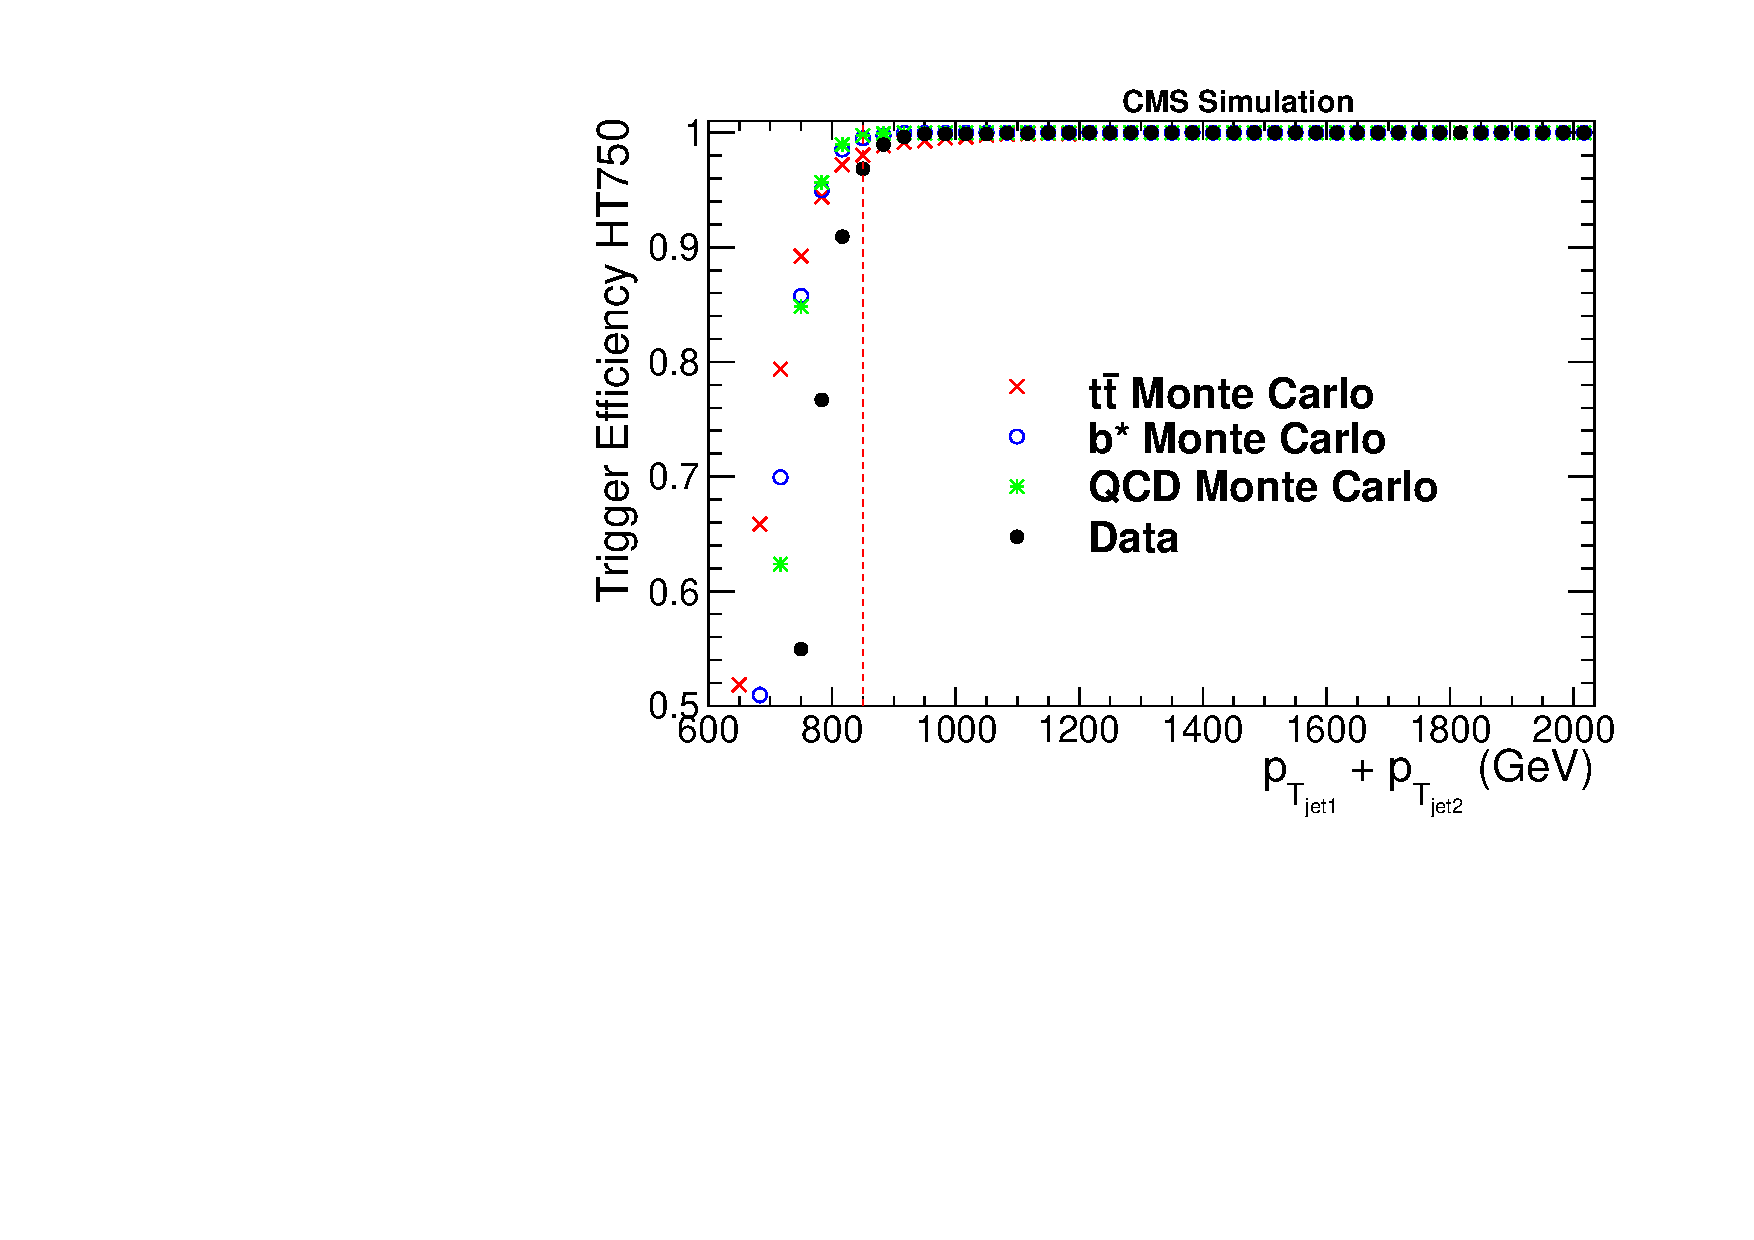
\includegraphics[width=0.9\textwidth]{AN-14-049/figs/Trigger_Comparison_Htdijet.pdf}
\caption{Trigger efficiency of \texttt{HLT\_HT750} measured as a function of the summed $\pt$ of the leading and sub-leading jets.  }
\label{figs:bsTrigger_Comparison_Ht}
\end{figure}

%\section{Signal Characteristics}
%\label{sec:bssigchar}
%\label{sec:bsGenBptCut}
%The $\bs$ quark of interest is very massive, and produces highly boosted top quarks.  The decay products of these top quarks become more collimated as the boost 
%increases.  When the top decays hadronically, we observe one merged jet over the two distinct jets that would be detected at a lower boost.  This jet has a 
%large characteristic radius and a distinct substructure.  This high energy jet merging is investigated in Figure \ref{figs:bstopmerge}.  Here, the `top candidate' 
%is just the leading jet in the event.  It is also required to be hemispherically separated from a Monte Carlo truth b jet.  This jet is generally a merged W %boson at low $\pt$ and a merged top at high $\pt$.
%The `W candidate' (used for the bottom plots) is assembled from the pair of generator level non-b quarks that are close to the W mass (within 2.0$\GeV$).  
%The central feature of this analysis is using this jet merging to discriminate signal from background.

%\begin{figure}[htcb]
%\centering
%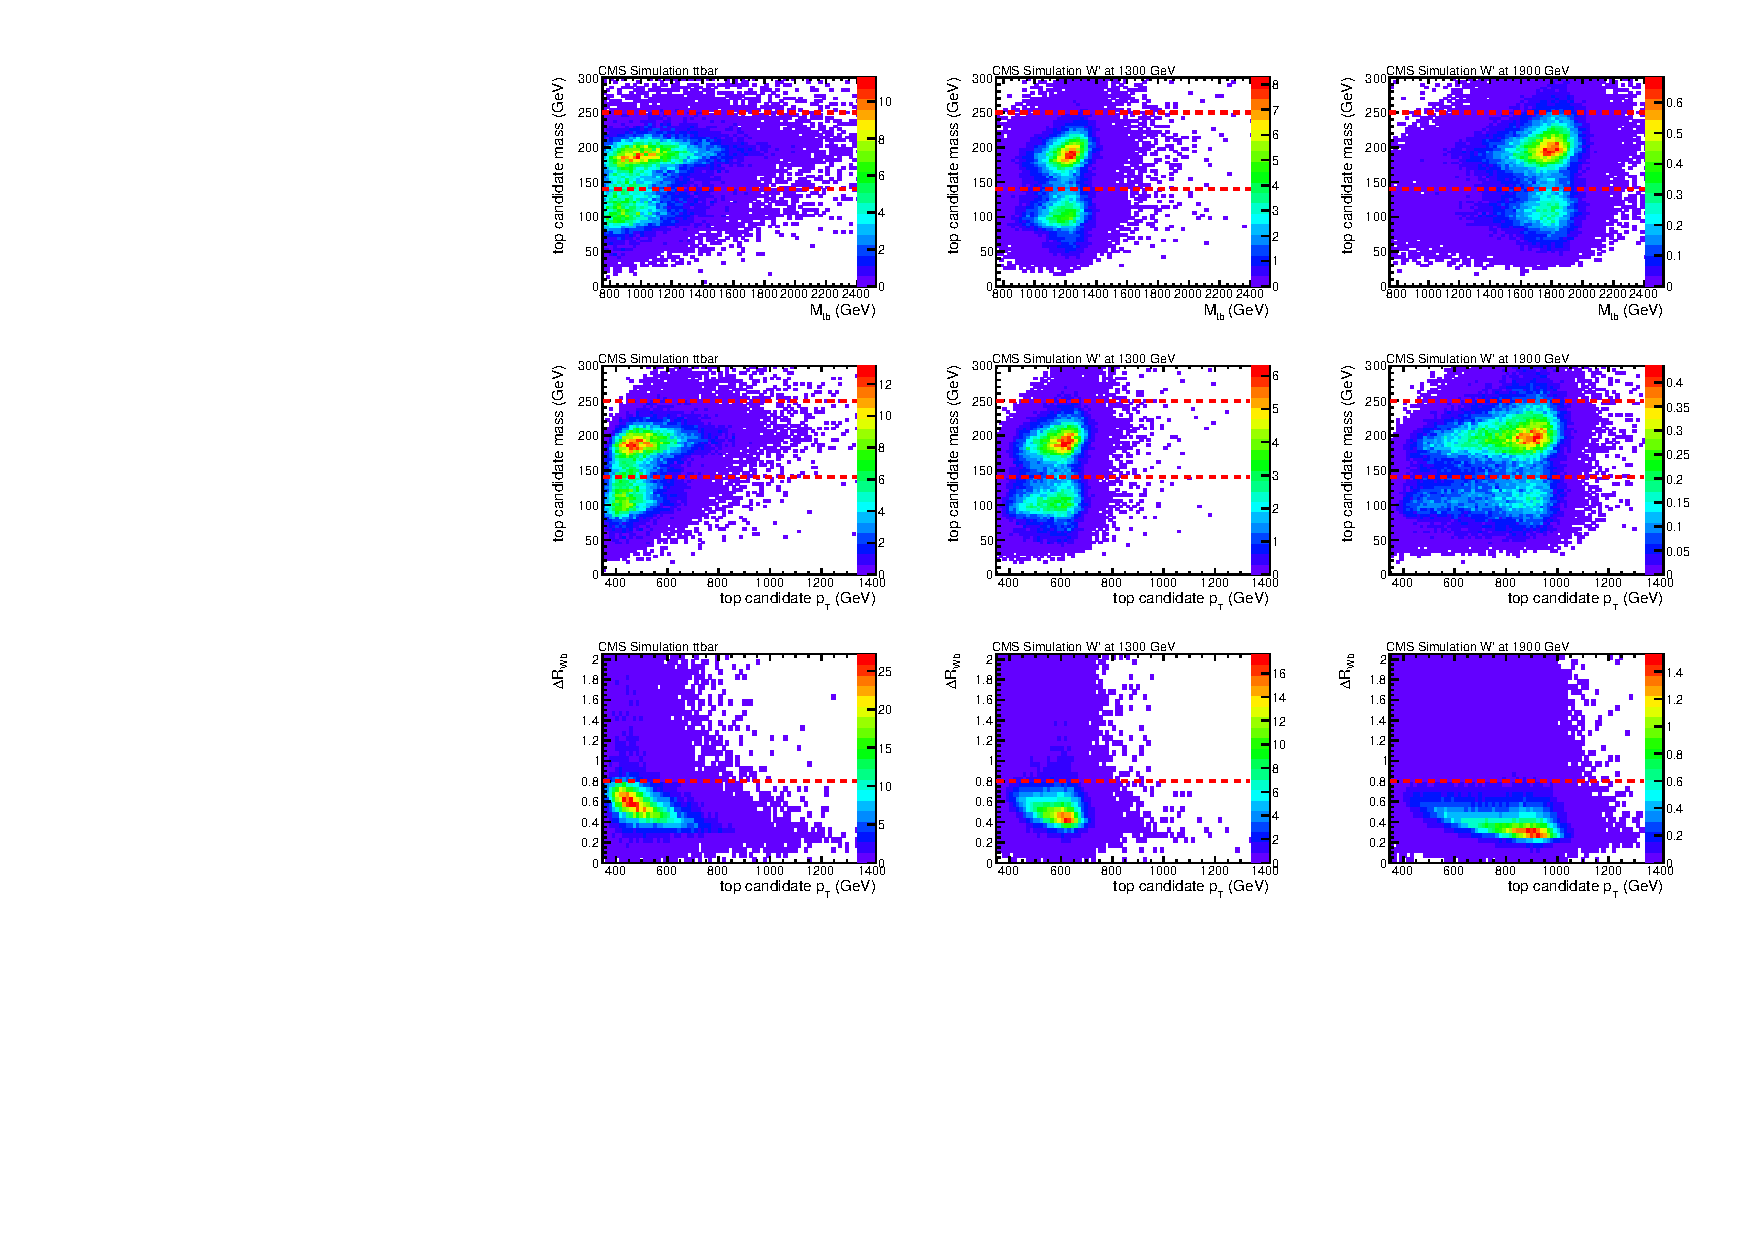
\includegraphics[width=0.9\textwidth]{AN-14-049/figs/topmerge.pdf}
%\caption{Investigation of top merging within Monte Carlo samples of interest.  $\ttbar$ (left) $\wpr_R$ Monte Carlo at 1300$\GeV$ (middle) $\wpr_R$ Monte Carlo %at 1900$\GeV$ (right).  The red lines on the top and middle plots indicate the top candidate mass cut in the full selection (see Section \ref{sec:bstoptagging}). % The red line on the bottom plots indicate the characteristic jet radius used to investigate fully merged top jets (see Section \ref{sec:bsreconstruction}).}
%\label{figs:bstopmerge}
%\end{figure}

%We place a generator level $\pt$ cut on the b quark from the $\wpr$ decay in the left-handed and mixed-coupling $\wpr$ samples (see Section \ref{sec:bssignal}).  
%To investigate the effect of this pre-selection, we look at the effect of an even tighter cut.  
%Figure \ref{figs:bsgenptcut} shows the ratio of generator level b $\pt$ cuts.  
%The denominator requires a generation level pt cut of 200 $\GeV$ and the numerator requires a generation level pt cut of 230 $\GeV$.  
%This ratio is parameterized in the $\pt$ of the CA8 jet that the generation particle is matched to ($\Delta R  < 0.5$ is used for matching).
%The turn on of this tighter cut is well below the analysis level cut of 370$~\GeV$.  Thus, the effect of the generation level b $\pt$ cut 
%on selections requiring the analysis level $\pt$ cut is negligible.  %

%\begin{figure}[Htcb]
%\centering
%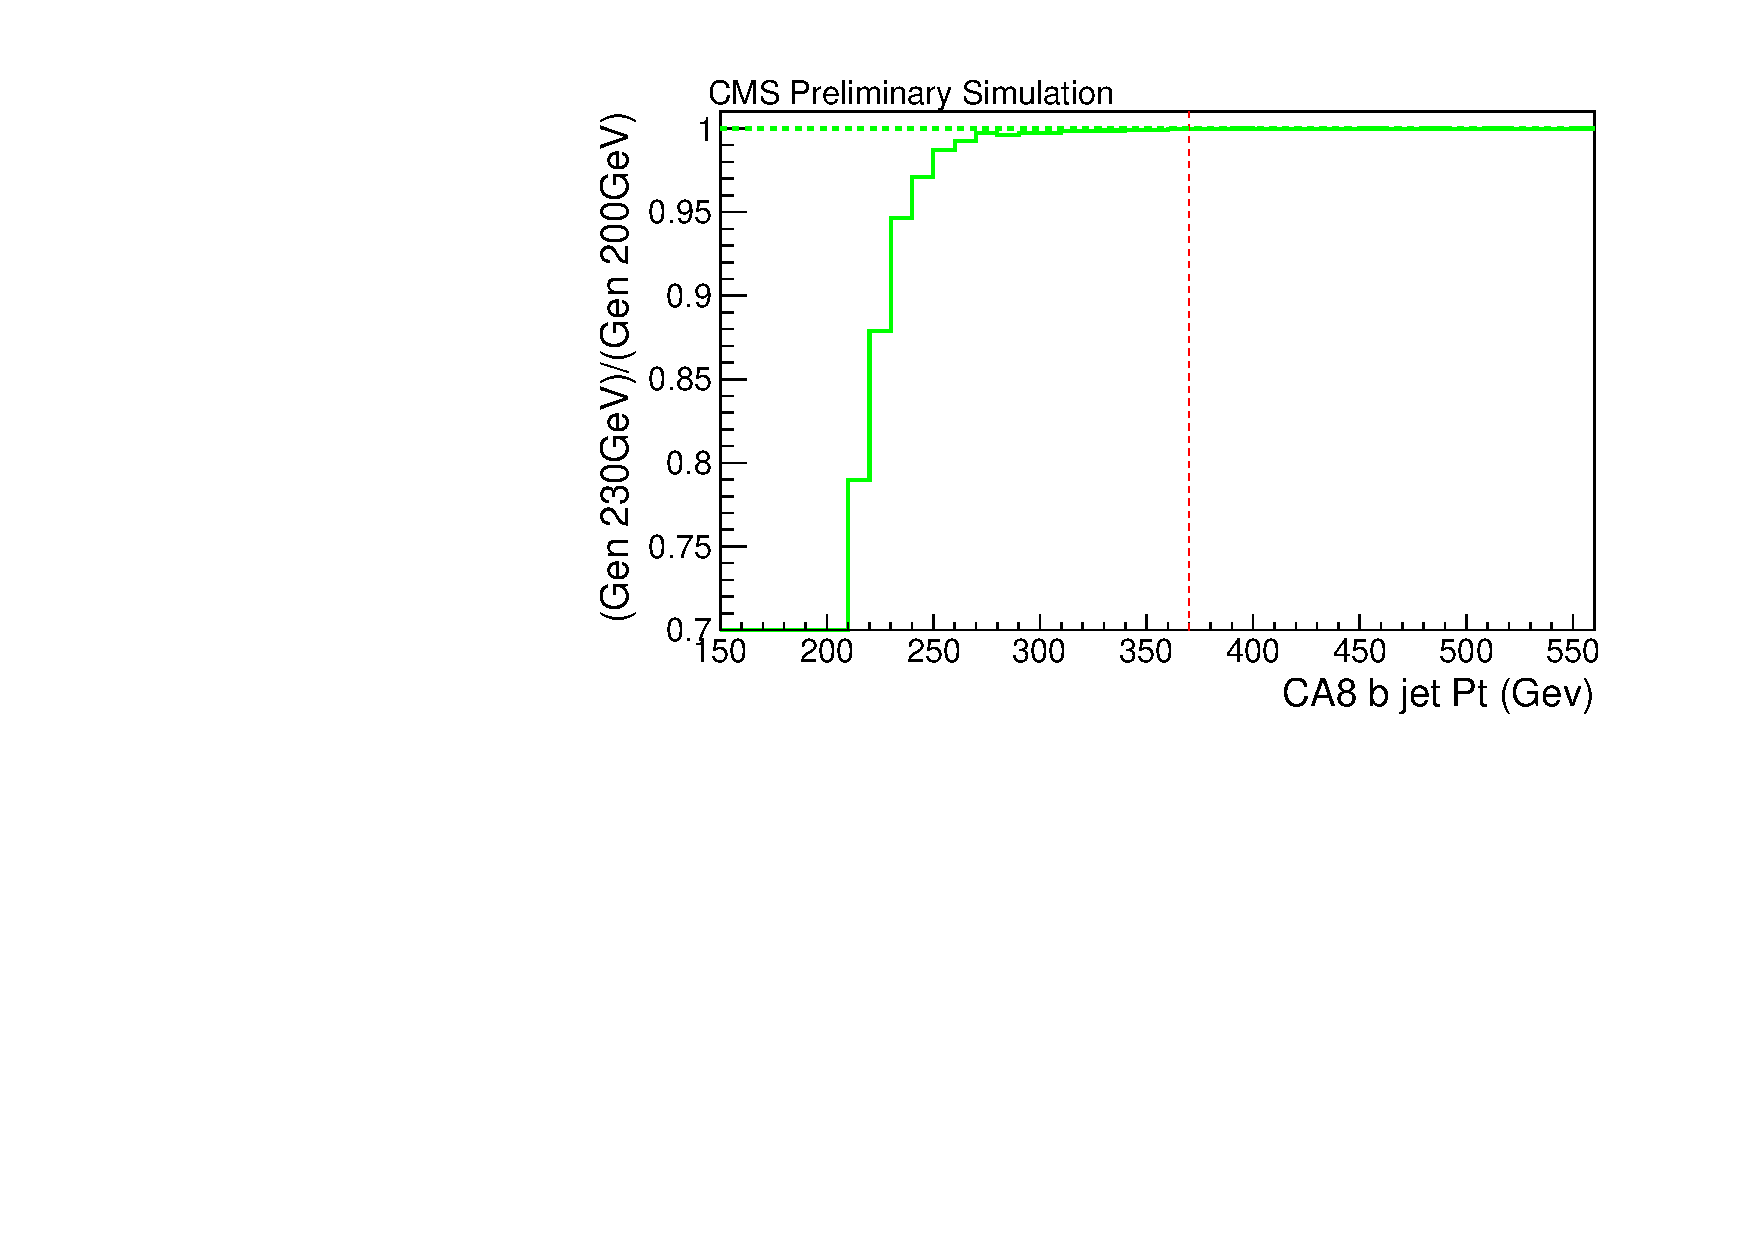
\includegraphics[width=1.0\textwidth]{AN-14-049/figs/bjetptcut.pdf}
%\caption{Ratio of CA8 $\pt$ using the generation level b pt cut of 230$~\GeV$ and 200$~\GeV$.  The red line is the analysis level $\pt$ cut of 370$~\GeV$.  The sample used for this study is $W`_{LR}$ at 1300$~\GeV$}
%\label{figs:bsgenptcut}
%\end{figure}


\section{Event Pre-selection}
\label{sec:bspre-selection}
The following pre-selection is applied:

\begin{itemize}
\item The event must have a good primary vertex as computed by a deterministic annealing filter (DAF)
($\vert z_\text{Primary Vertex}\vert < 24$ cm, $N_\text{DOF} > 6$).
\item Two jets with $|y| < 2.4$
\item Exactly two jets with $\pt > 150~\GeV$
\item Leading Jet \& Sub-leading Jet $\pt > 425~\GeV$
\item Loose Particle Flow jet identification \cite{jetid} is applied
\item Beam background events are removed using the following requirements:
        \begin{itemize}
        \item In events with at least 10 tracks, a minimum of 25\% of
          these tracks must be high purity tracks.
        \end{itemize}
\end{itemize}

Here we do not include the $|\Delta y|$ discrimination used in the $\wpr$ search due to the fact that the expected 
$\bs$ mass exclusion point is lower, and this cut is highly energy dependent.  


%\section{$\ttbar$ $\pt$ Re-weighting}
%\label{sec:bsttptrw}
%In order to correct for known differences in the top $\pt$ spectrum between data and $\ttbar$ Monte Carlo, we re-weight Monte Carlo using the Generator level $\pt%$ of the top and anti-top with the recommended prescription.  
%With $p_{T_{t}}$ and $p_{T_{\overline{t}}}$ being the generator $\pt$ of the top and anti-top respectively, the scale factor applied to each event in the $\ttbar%$ Monte Carlo expectation is:%
%\begin{eqnarray}
%SF =\sqrt{e^{0.156-.00137p_{T_{t}}} \times e^{0.156-.00137p_{T_{\overline{t}}}}}
%\end{eqnarray}
%Although this procedure was not designed for the kinematic range in our analysis, we prefer to use the prescription as it is more consistent with our measurement of the $\ttbar$ normalization (see Section \ref{sec:bsttbarsideband}).


\section{Pileup Correction}
\label{sec:bspileup}
We re-weight our Monte Carlo samples to account for differences due to pileup using the recommended procedure (see Section~\ref{sec:pileup}).  
Figure \ref{figs:bsnpvweight} shows the distribution of reconstructed primary vertices in data, $\ttbar$,
and signal Monte Carlo before and after the re-weighting has been applied. The pileup correction has very little effect on the eventual $\mathrm{M_{tW}}$ 
full selection, as 
seen in Figure \ref{figs:bspileup3}, for $\bs_R$ signal Monte Carlo at the 1300$~\GeV$ mass point. Similarly, there is little effect 
$\ttbar$ Monte Carlo as can be seen in Figure \ref{figs:bspileup3ttbar}.  
A study has been conducted to investigate the effect of the suggested systematic uncertainty of 5\% on the minbias cross-section as can be seen in Section \ref{sec:bssystematics}.  


\begin{figure}
\begin{center}
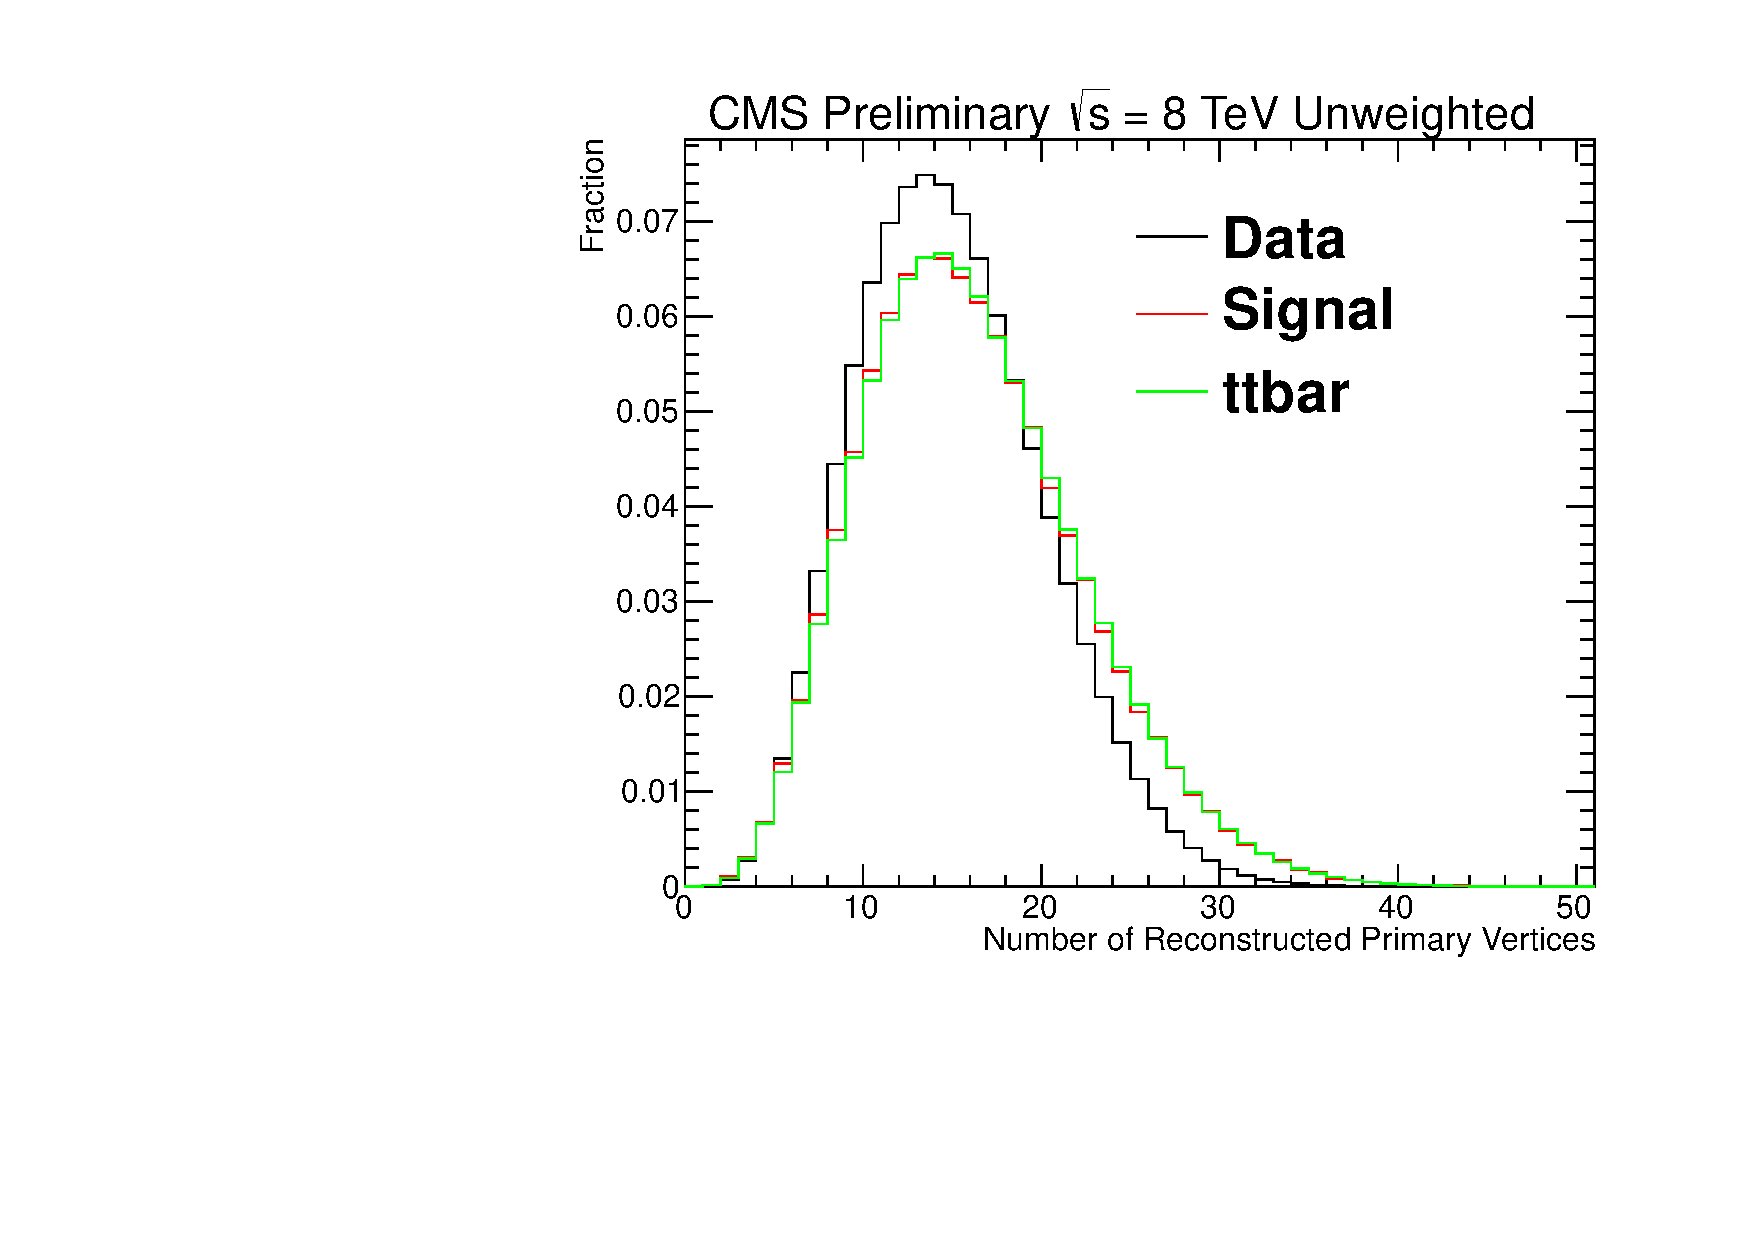
\includegraphics[width=0.7\linewidth]{AN-14-049/figs/npvuw.pdf}\\
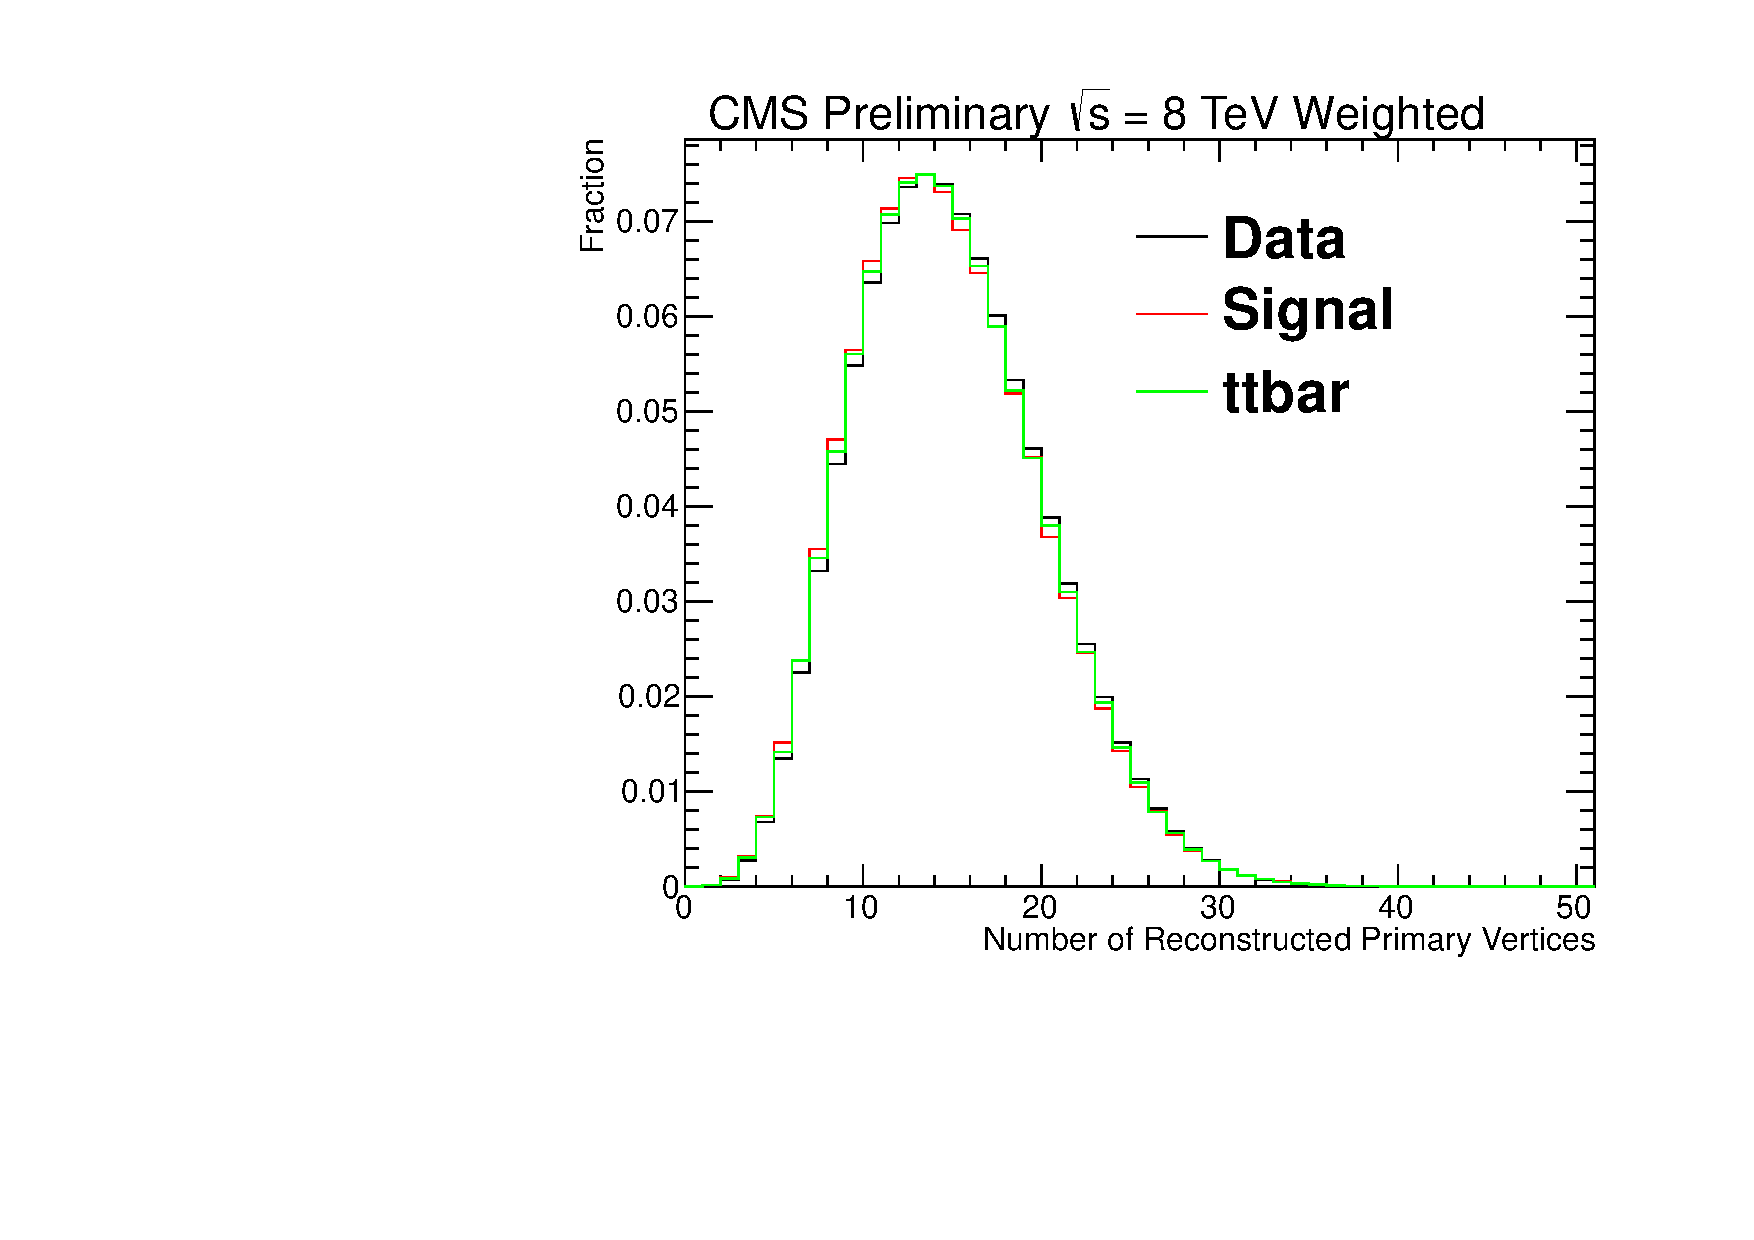
\includegraphics[width=0.7\linewidth]{AN-14-049/figs/npvw.pdf}
\end{center}
\caption{Number of reconstructed primary vertices before pileup re-weighting (top) and after pileup re-weighting (bottom).  Here, no analysis cuts have been applied and the signal is $\bs_R$ 1000$~\GeV$}
\label{figs:bsnpvweight}
\end{figure}

\begin{figure}[htcb]
\centering
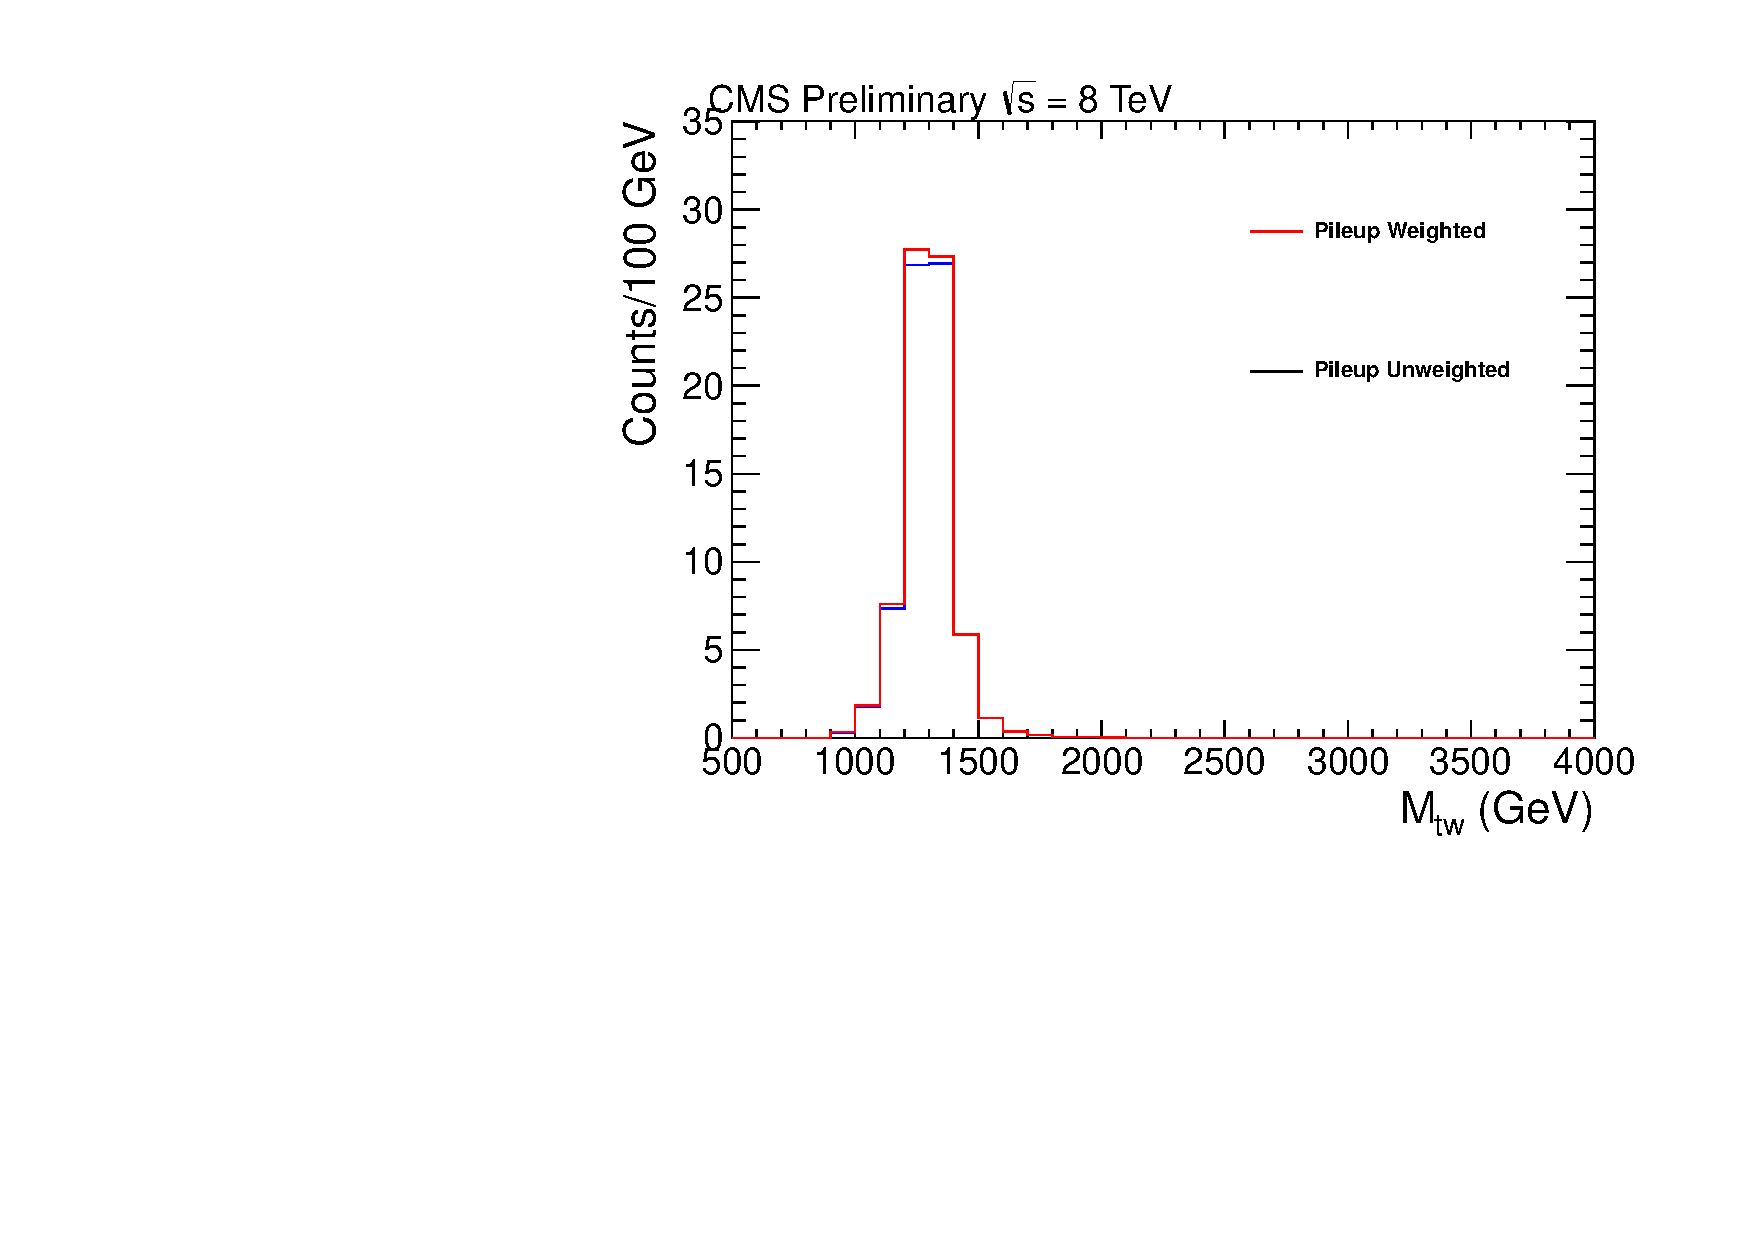
\includegraphics[width=0.9\textwidth]{AN-14-049/figs/Signal_M1300_PileupComp.pdf}
\caption{Effect of pileup re-weighting on the right-handed $\bs$ Signal Monte Carlo.}
\label{figs:bspileup3}
\end{figure}

\begin{figure}[htcb]
\centering
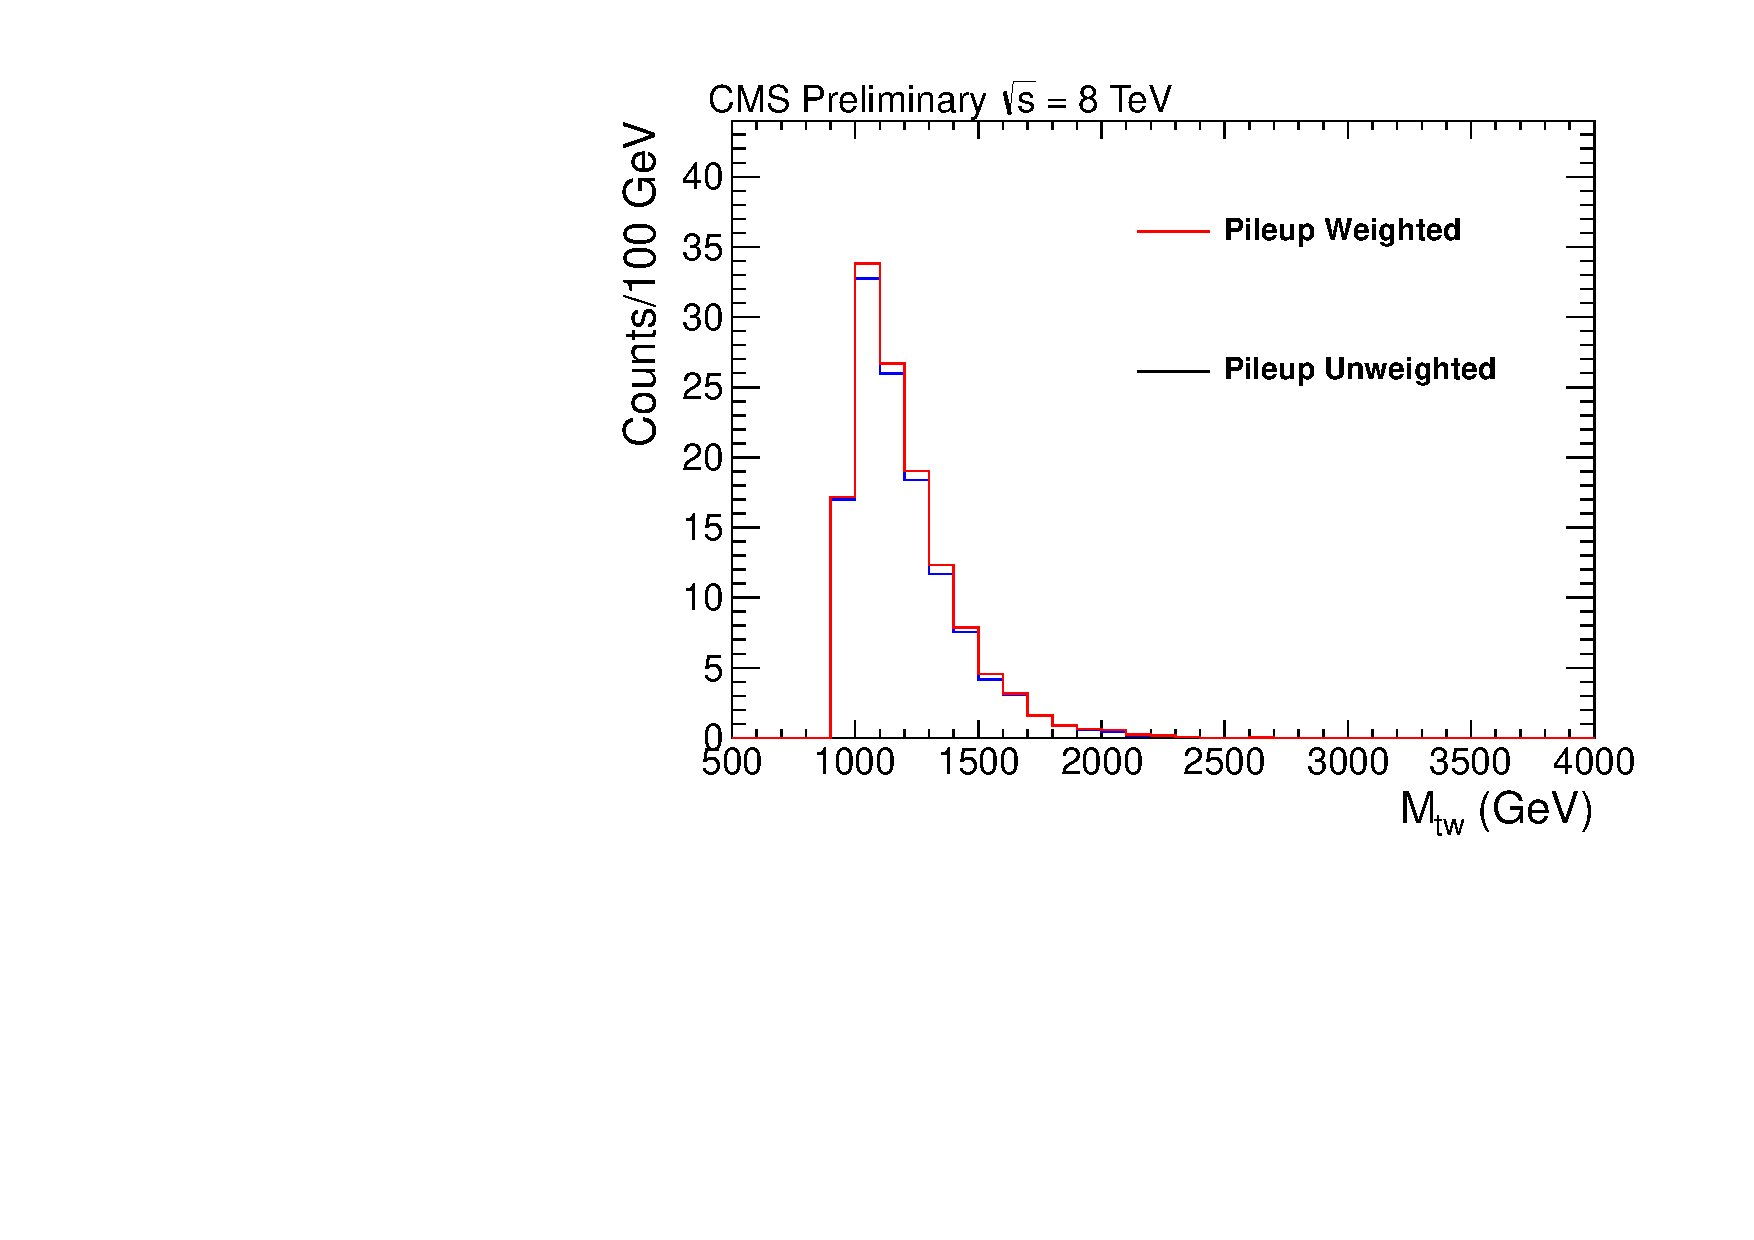
\includegraphics[width=0.9\textwidth]{AN-14-049/figs/TTbar_PileupComp.pdf}
\caption{Effect of pileup re-weighting on the $\ttbar$ Monte Carlo.}
\label{figs:bspileup3ttbar}
\end{figure}



\section{Combined CMS Top Tagging Algorithm}
\label{sec:bstoptagging}
\label{sec:bssubjetSF}
The CMS top tagging algorithm is described in detail in Section~\ref{sec:toptagging}.
Figure \ref{figs:bsNsubCOMP} shows $\tau_3/\tau_2$ comparison using signal and QCD Monte Carlo samples.  We use the standard operating point of $\tau_3/\tau_2 < 0.55$ in the full selection.
Figure \ref{figs:bsBtagCOMP} shows the maximum subjet CSV b discriminant comparison using signal and QCD Monte Carlo samples.  We use the standard CSV working point $SJ_{CSVMAX} > 0.679$.

\begin{figure}[htcb]
\begin{center}
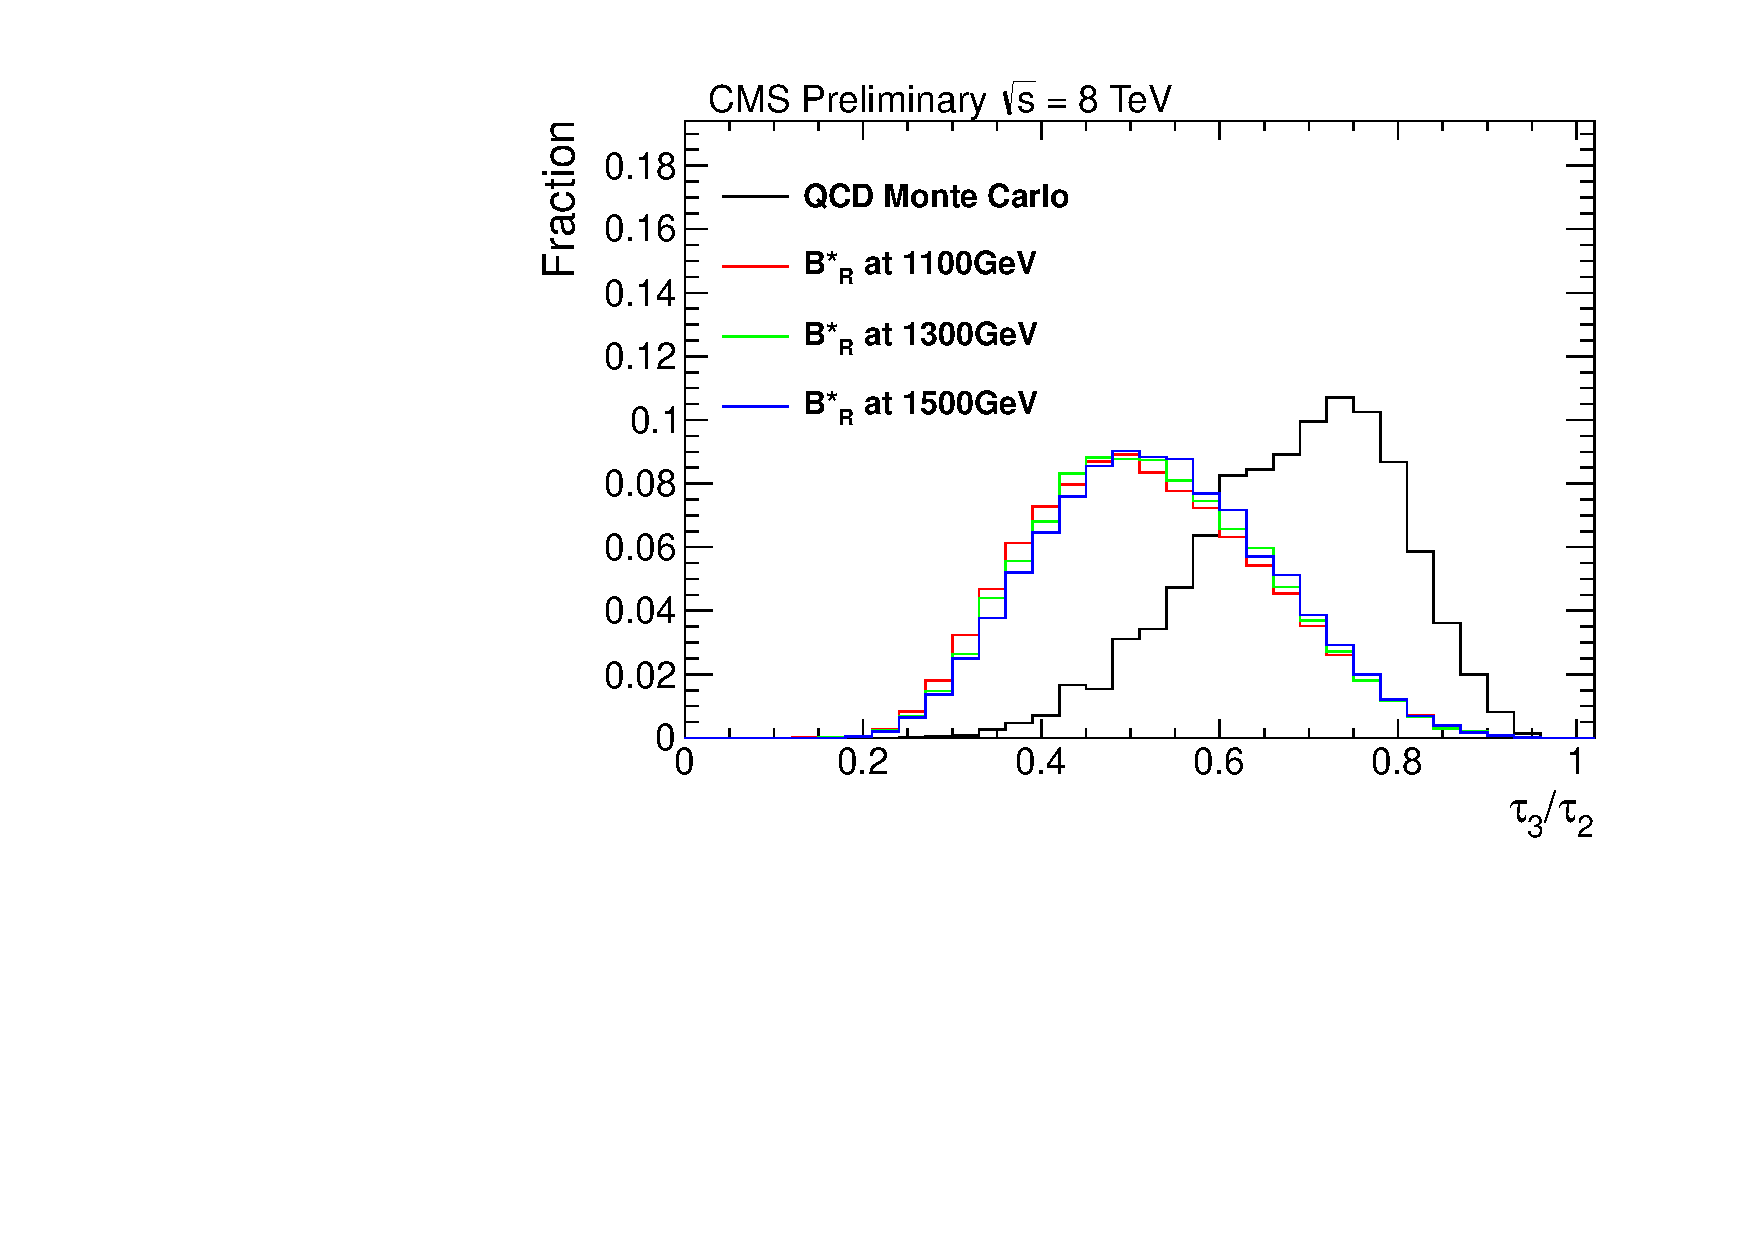
\includegraphics[width=0.7\textwidth]{AN-14-049/figs/tau32rightCompqcdandsignal.pdf}\\
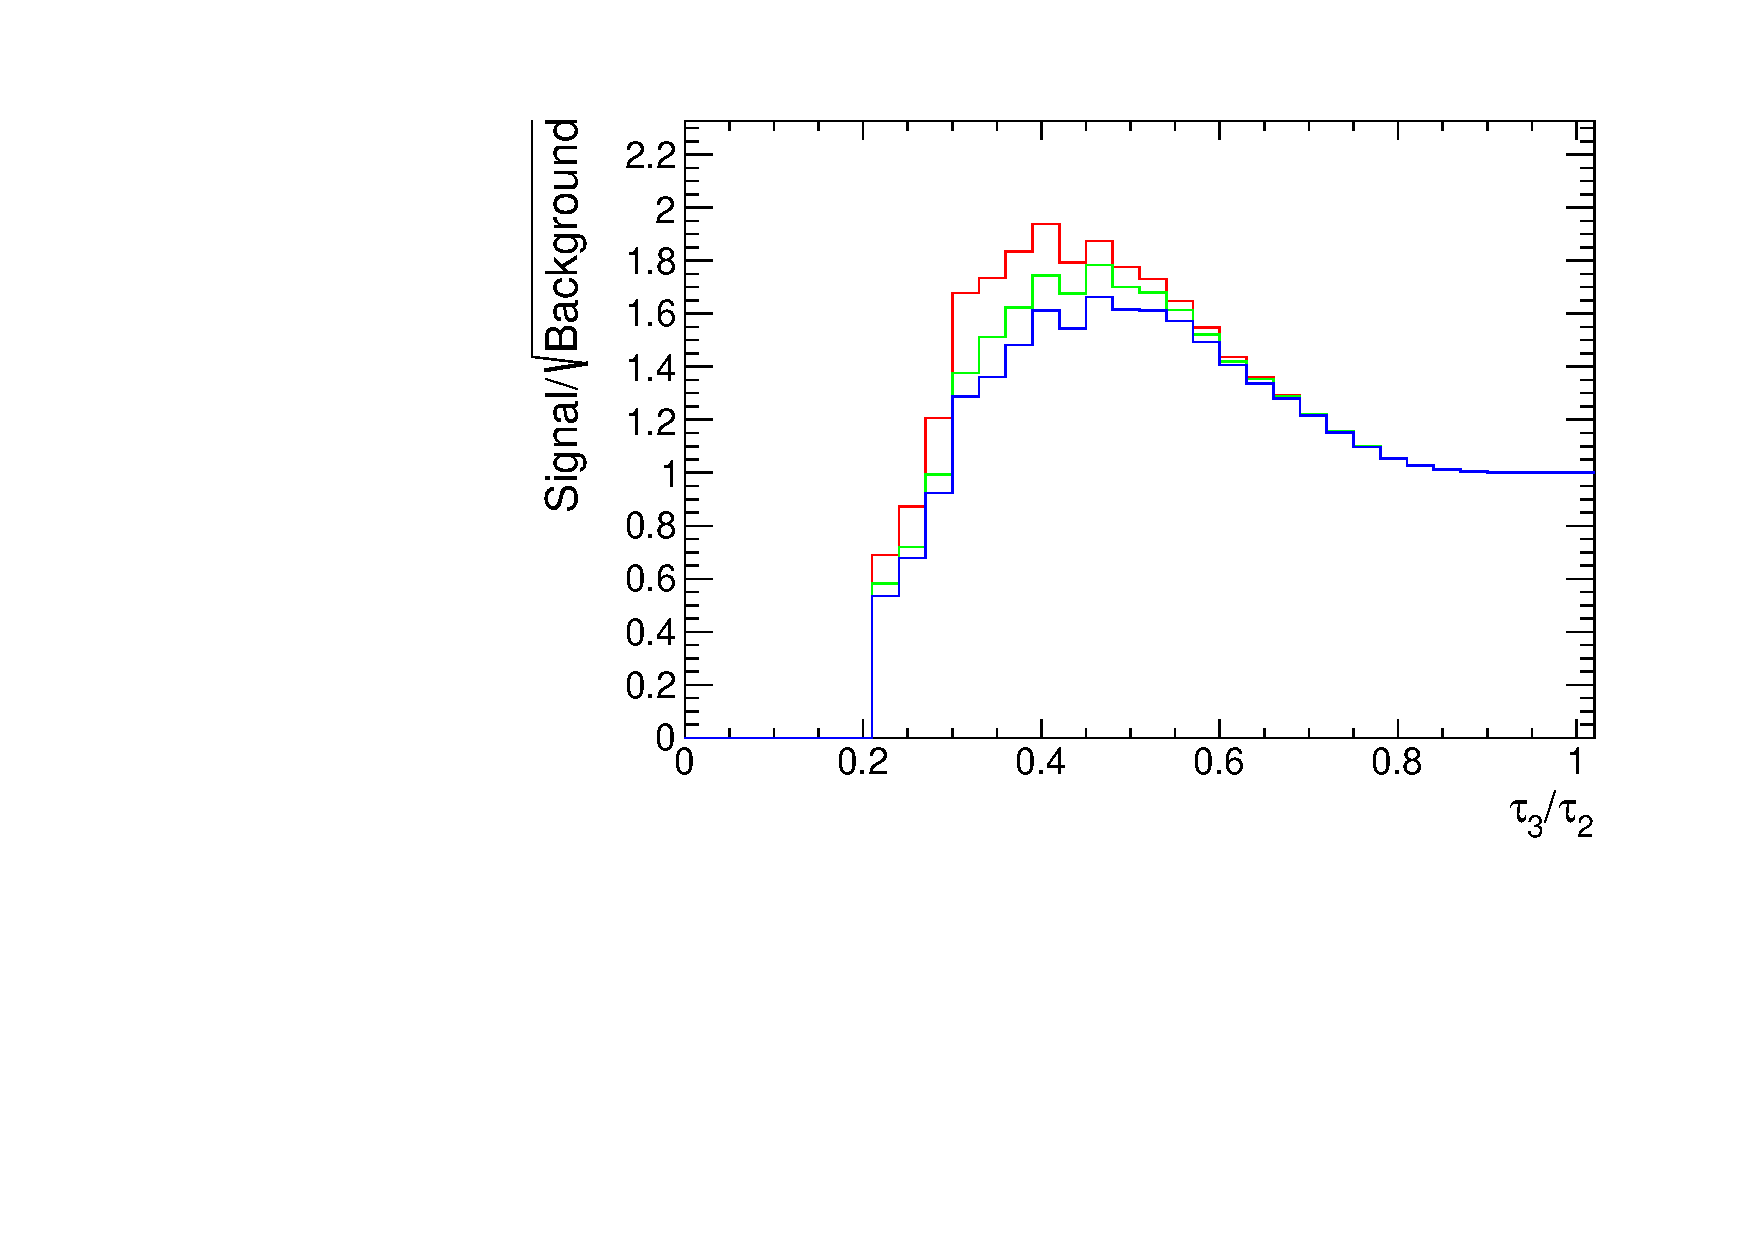
\includegraphics[width=0.7\textwidth]{AN-14-049/figs/tau32rightSNRqcdandsignal.pdf}
\caption{
$\tau_3/\tau_2$ distributions in Signal and QCD Monte Carlo samples (top).  The selection here includes the full signal region with the exception of subjet b-tagging in order to preserve QCD Monte Carlo statistics.  Plot of Signal/$\sqrt{\text{Background}}$ (bottom), derived from the top plot.
}
\label{figs:bsNsubCOMP}
\end{center}
\end{figure}




\begin{figure}[htcb]
\begin{center}
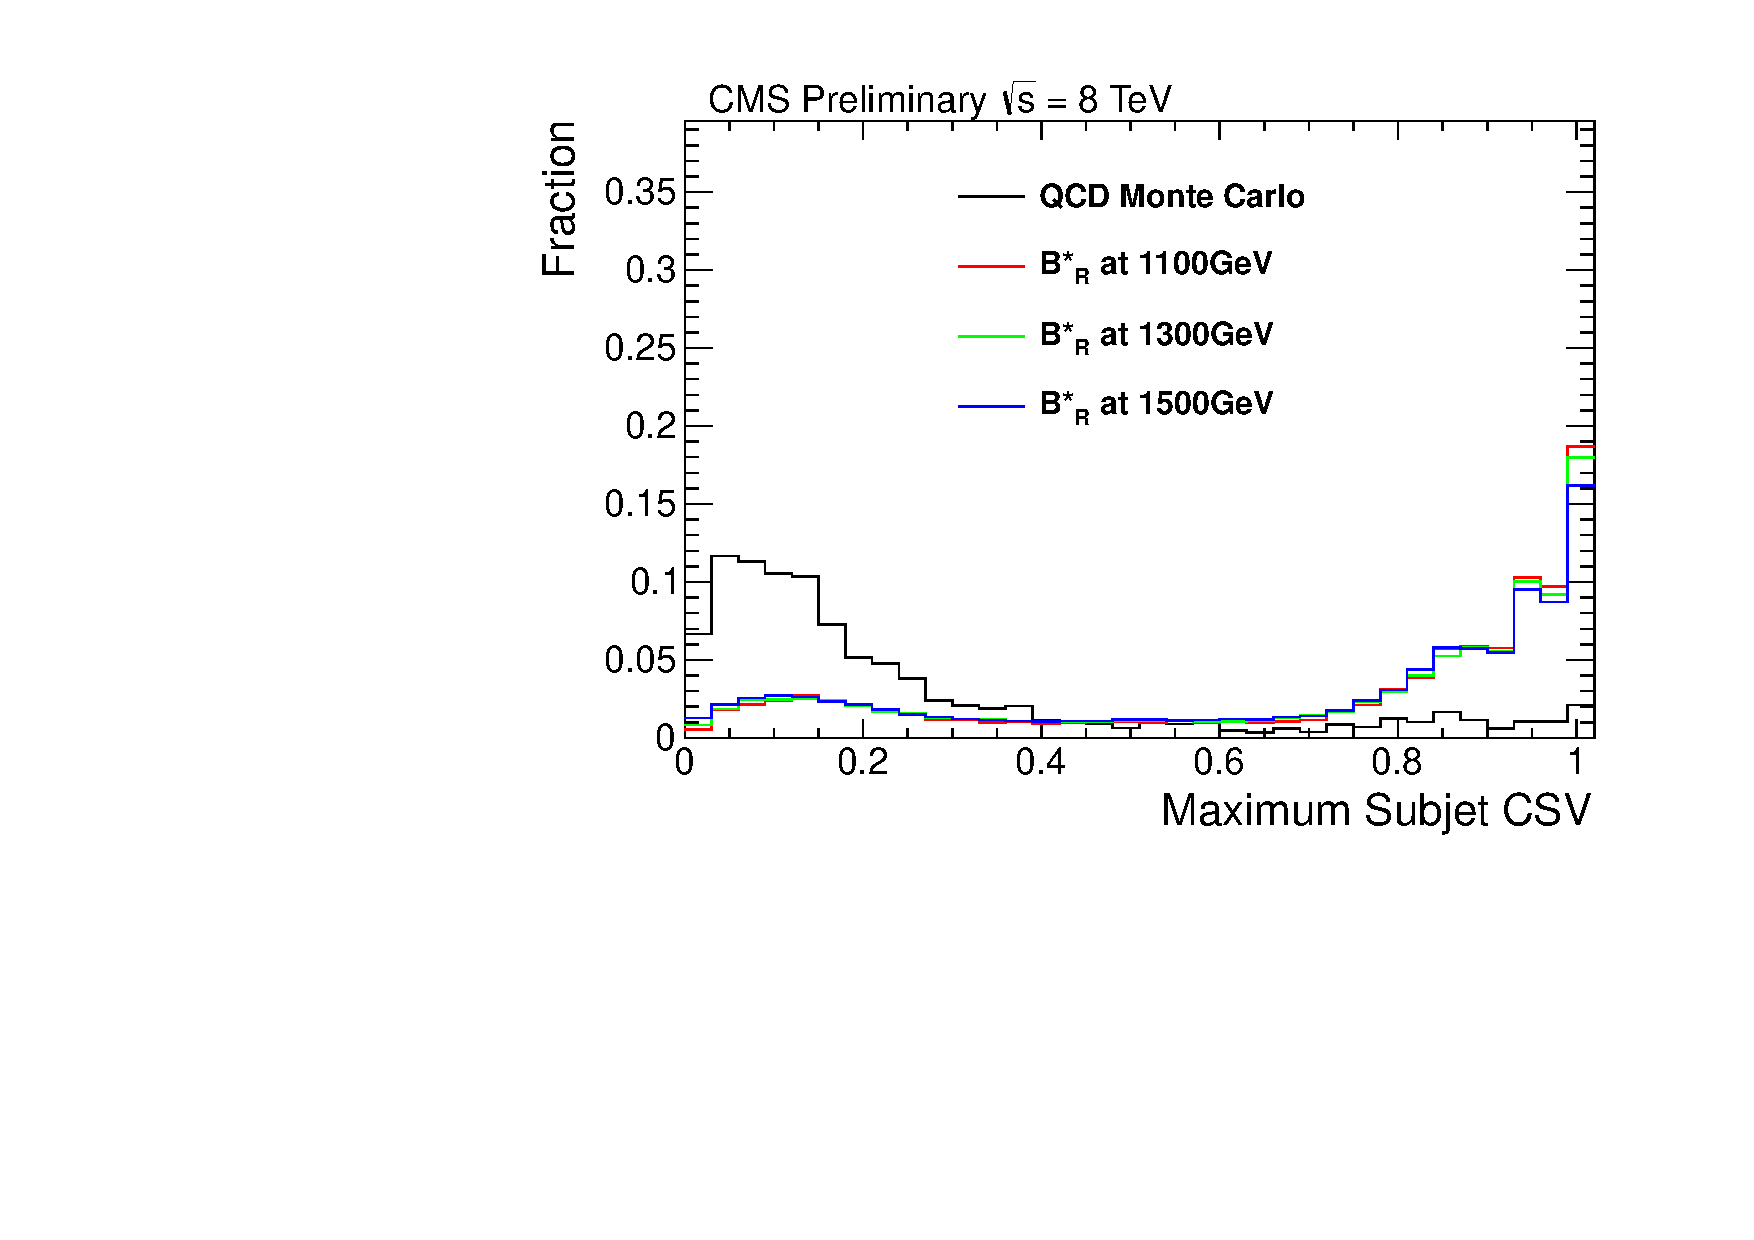
\includegraphics[width=0.7\textwidth]{AN-14-049/figs/TopBDiscsjmaxCSVrightCompqcdandsignal.pdf}\\
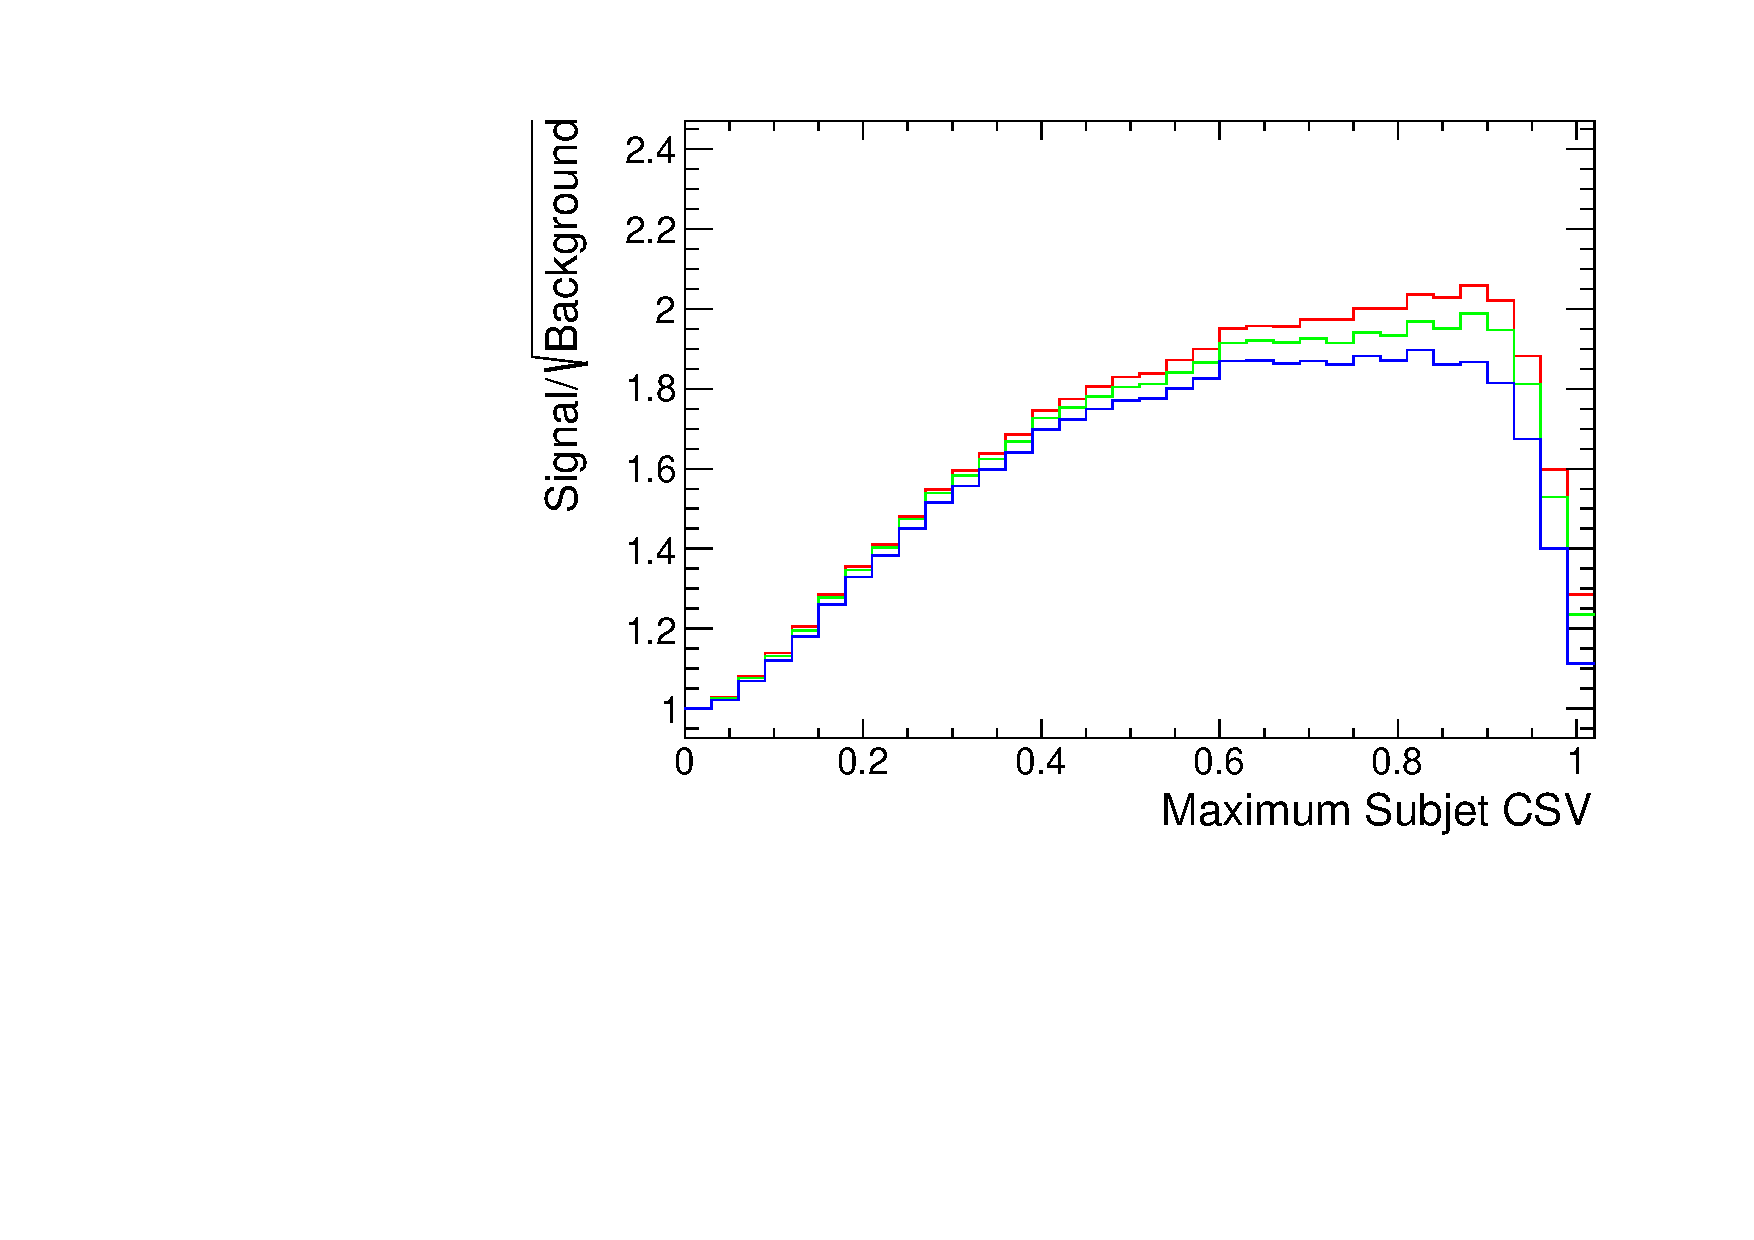
\includegraphics[width=0.7\textwidth]{AN-14-049/figs/TopBDiscsjmaxCSVrightSNRqcdandsignal.pdf}
\caption{
Maximum subjet CSV distributions in Signal and QCD Monte Carlo samples (top).  Plot of Signal/$\sqrt{\text{Background}}$ (bottom), derived from the top plot. 
}
\label{figs:bsBtagCOMP}
\end{center}
\end{figure}


\section{W Jet Identification}
\label{sec:bswtagging}
The W boson daughter if the $\bs$ quark will also be boosted.  Just as the CMS top tagging algorithm discriminates signal from background 
using the merged top jet, the boosted W boson tagging discriminates signal from background by using a merged W jet.  For this we constrain the 
jet mass to the W boson range, and use the N-subjettiness algorithm.  To identify the two subjets of the W boson, the N-subjettiness variable used is 
$\tau_{2}/\tau_{1}$ due to the fact that the jet energy is more consistent with two subjets than one.
 
\begin{itemize}
\item {\bf Jet Mass}  $\mathrm{\boldmath 70~\GeV < m_{\text{jet}} < 100~\GeV}$ - The mass of the CA jet is required to be consistent with the W boson mass. 
\item {\bf N-subjettiness} $\mathrm{\boldmath \tau_{2}/\tau_{1} < 0.5}$  - The ratio of the N-subjettiness variables $\tau_{2}$ and $\tau_{1}$ should be low, as the W jet is more consistent with two subjets than one.
\end{itemize}

\section{Reconstruction of $\bs$ invariant mass}
\label{sec:bsfullselection}
The full selection for the reconstruction of the $\bs$ invariant mass then includes the following offline cuts.
\begin{itemize}
\item One jet with $\pt > 425~\GeV$ with the CMS top tagging algorithm as well as subjet b-tagging and N-subjettiness discrimination.
\item One jet with $\pt > 425~\GeV$ with a boosted W tag
\item $|\Delta \phi| > \pi/2$ between the two jets
\end{itemize}
After this selection, the b* invariant mass is reconstructed using the top-W candidate mass ($\mathrm{M_{tW}}$).
The cutflow for this selection in data, $\ttbar$ Monte Carlo, and $\bs$ signal Monte Carlo can be found in Table \ref{table:bsCutflow}.
Figure \ref{figs:bsGCFS} shows this full selection in signal Monte Carlo for various $\bs$ masses.  



\begin{sidewaystable}
\begin{center}
\begin{small}
\begin{tabular}{|c||c|c|c|c|c|c|c|c|c|c|}
\multicolumn{8}{c}{Cutflow} \\
\hline
\bf{Sample} & \bf{$\geq 2 jets$} & \bf{$exactly 2 jets$} & \bf{$\pt$} & \bf{$M_{top}$} & \bf{$Nsubjets$} &  \bf{$Minmass$}  & $\tau_3/\tau_2$  & $SJ_{CSVMAX}$  & \bf{$M_{W}$} & $\tau_2/\tau_1$ \\ 
\hline\hline
Data & 18868018 & 13854873 & 3545312 & 1047669 & 593104 & 337754 & 39409 & 7334 & 800 & 318\\ 
\hline
QCD & --- & --- & --- & --- & --- & --- & --- & --- & --- & 211\\ 
\hline
ttbar & 13214 & 10453 & 3533 & 2683 & 2338 & 2146 & 1295 & 934 & 174 & 129\\ 
\hline
M($b*_{R}$) = 800 & 3930 & 3334 & 388 & 233 & 196 & 175 & 99 & 67 & 40 & 33\\ 
\hline
M($b*_{R}$) = 900 & 4300 & 3782 & 854 & 445 & 385 & 345 & 212 & 149 & 106 & 91\\ 
\hline
M($b*_{R}$) = 1000 & 3136 & 2769 & 1407 & 789 & 681 & 614 & 381 & 276 & 217 & 183\\ 
\hline
M($b*_{R}$) = 1100 & 1976 & 1730 & 1191 & 732 & 631 & 572 & 350 & 251 & 192 & 161\\ 
\hline
M($b*_{R}$) = 1200 & 1183 & 1031 & 808 & 538 & 460 & 421 & 254 & 180 & 137 & 114\\ 
\hline
M($b*_{R}$) = 1300 & 705 & 607 & 507 & 357 & 304 & 280 & 166 & 116 & 88 & 73\\ 
\hline
M($b*_{R}$) = 1400 & 429 & 365 & 318 & 232 & 196 & 181 & 105 & 72 & 55 & 45\\ 
\hline
M($b*_{R}$) = 1500 & 255 & 216 & 193 & 145 & 121 & 112 & 64 & 43 & 33 & 27\\ 
\hline
M($b*_{R}$) = 1600 & 155 & 131 & 118 & 91 & 76 & 70 & 39 & 26 & 19 & 16\\ 
\hline
M($b*_{R}$) = 1700 & 97 & 80 & 74 & 57 & 47 & 43 & 24 & 16 & 12 & 9\\ 
\hline
M($b*_{R}$) = 1800 & 59 & 49 & 45 & 35 & 29 & 27 & 15 & 9 & 7 & 5\\ 
\hline
M($b*_{R}$) = 1900 & 37 & 30 & 28 & 22 & 18 & 17 & 9 & 6 & 4 & 3\\ 
\hline
M($b*_{R}$) = 2000 & 23 & 19 & 18 & 14 & 12 & 10 & 5 & 3 & 2 & 2\\ 
\hline
M($b*_{L}$) = 800 & 3855 & 3259 & 374 & 227 & 179 & 159 & 84 & 55 & 31 & 26\\ 
\hline
M($b*_{L}$) = 900 & 4223 & 3712 & 838 & 472 & 376 & 330 & 186 & 129 & 88 & 75\\ 
\hline
M($b*_{L}$) = 1000 & 3103 & 2744 & 1356 & 810 & 637 & 555 & 309 & 221 & 173 & 147\\ 
\hline
M($b*_{L}$) = 1100 & 1959 & 1722 & 1172 & 757 & 601 & 532 & 292 & 204 & 157 & 131\\ 
\hline
M($b*_{L}$) = 1200 & 1180 & 1028 & 797 & 548 & 436 & 389 & 210 & 144 & 109 & 91\\ 
\hline
M($b*_{L}$) = 1300 & 703 & 606 & 503 & 365 & 290 & 262 & 138 & 93 & 70 & 58\\ 
\hline
M($b*_{L}$) = 1400 & 423 & 361 & 313 & 235 & 187 & 170 & 87 & 58 & 44 & 36\\ 
\hline
M($b*_{L}$) = 1500 & 254 & 215 & 191 & 146 & 116 & 105 & 53 & 34 & 25 & 21\\ 
\hline
M($b*_{L}$) = 1600 & 155 & 130 & 117 & 92 & 73 & 66 & 33 & 20 & 15 & 12\\ 
\hline
M($b*_{L}$) = 1700 & 95 & 79 & 73 & 58 & 45 & 41 & 20 & 12 & 9 & 7\\ 
\hline
M($b*_{L}$) = 1800 & 59 & 49 & 45 & 36 & 28 & 25 & 12 & 7 & 5 & 4\\ 
\hline
M($b*_{L}$) = 1900 & 37 & 30 & 28 & 23 & 18 & 16 & 8 & 4 & 3 & 2\\ 
\hline
M($b*_{L}$) = 2000 & 23 & 19 & 18 & 14 & 11 & 10 & 5 & 3 & 2 & $<1$\\ 
\hline

\end{tabular}
\caption{Cutflow Table.  Table reads left to right where the current column implies the previous cuts.  QCD expectation is only recorded for the full selection, 
due to the fact that the background estimate is only valid after top tagging.  The first column implies the $\pt>150~\GeV$ preselection for any jet.  The second column additionally represents the delta phi selection between the leading jets.  
The column labeled $\pt$ represents the $\pt$ cut placed on both leading jets.}
\label{table:bsCutflow}
\end{small}
\end{center}
\end{sidewaystable}


\begin{figure}[htcb]
\begin{center}
\subfigure{\label{figs:bsGCFSright}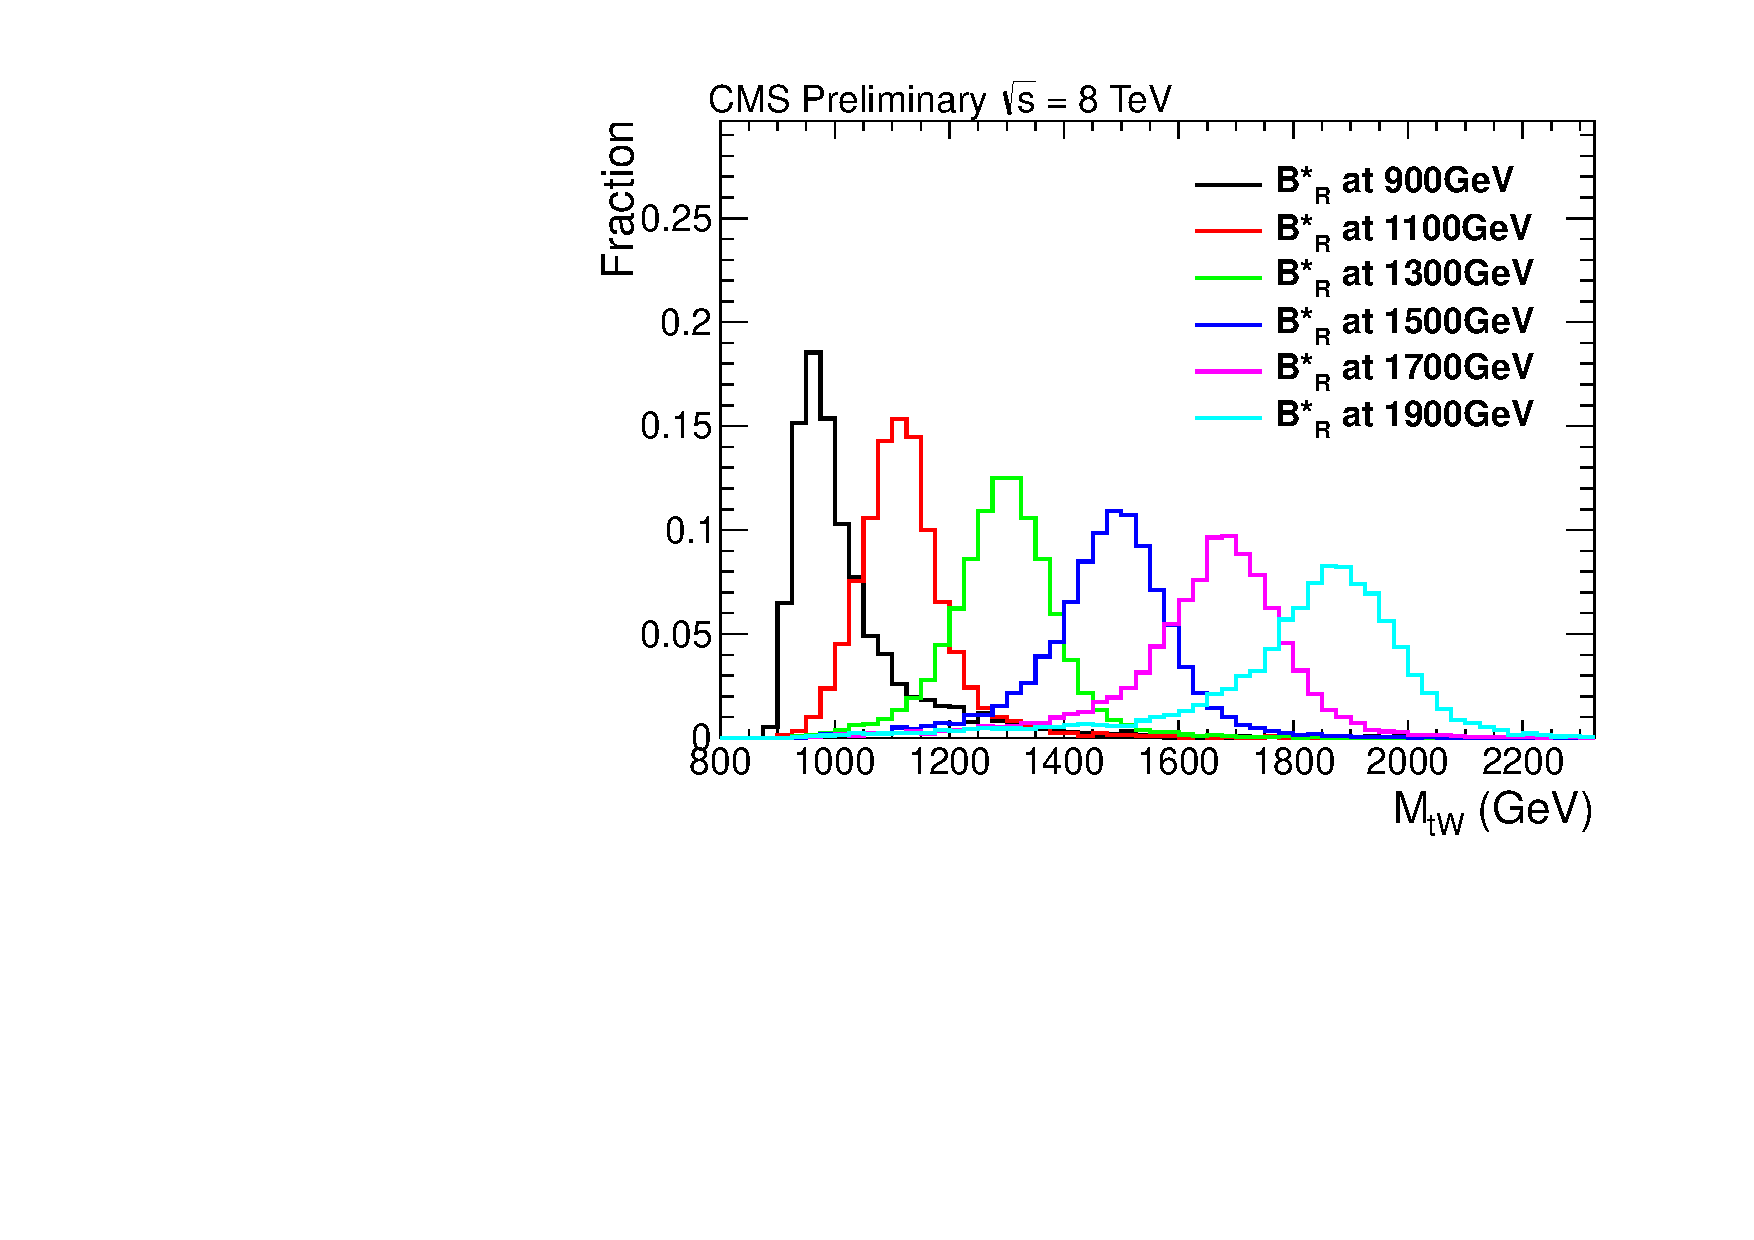
\includegraphics[width=1.0\textwidth]{AN-14-049/figs/SignalMCFSrightcomparison.pdf}}\\
\subfigure{\label{figs:bsGCFSleft}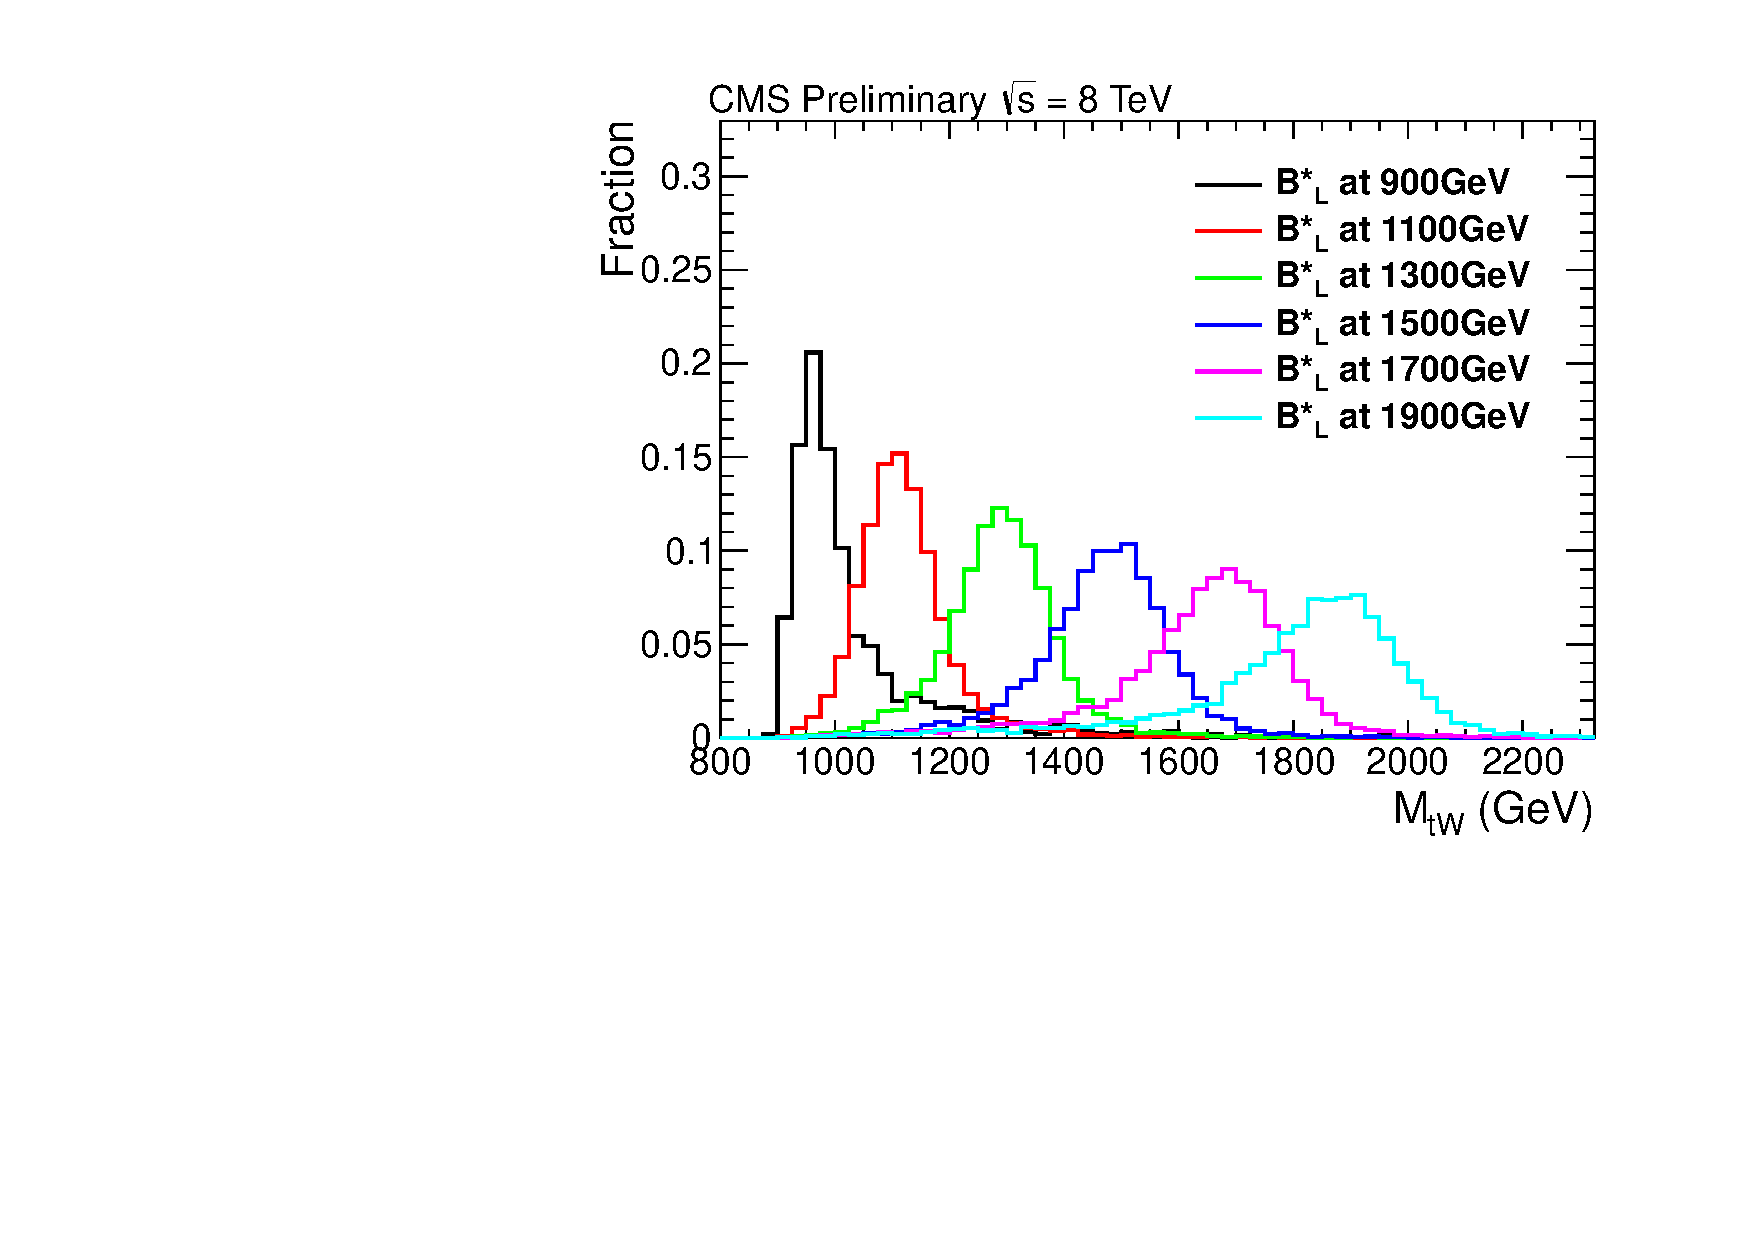
\includegraphics[width=1.0\textwidth]{AN-14-049/figs/SignalMCFSleftcomparison.pdf}}
\caption{
Full selection applied to $\bs_{R}$ (top) and $\bs_{L}$ (bottom-left).
}
\label{figs:bsGCFS}
\end{center}
\end{figure}

\clearpage
